\section*{Discretizzazione monodimensionale\\ del tessuto mammario}
Si consideri il tessuto mammario formato da una distribuzione in parallelo di diversi tessuti. All'interno di esso è presente una massa tumorale da trattare attraverso termoablazione.\\Per ridurre la complessità del problema si effettui un'analisi monodimensionale lungo l'asse verticale x, passante lungo il tumore e avente origine in corrispondenza di quest'ultimo esattamente come mostrato in \textbf{Fig.\ref{sistema}}.

\begin{figure}[H]
    \centering
    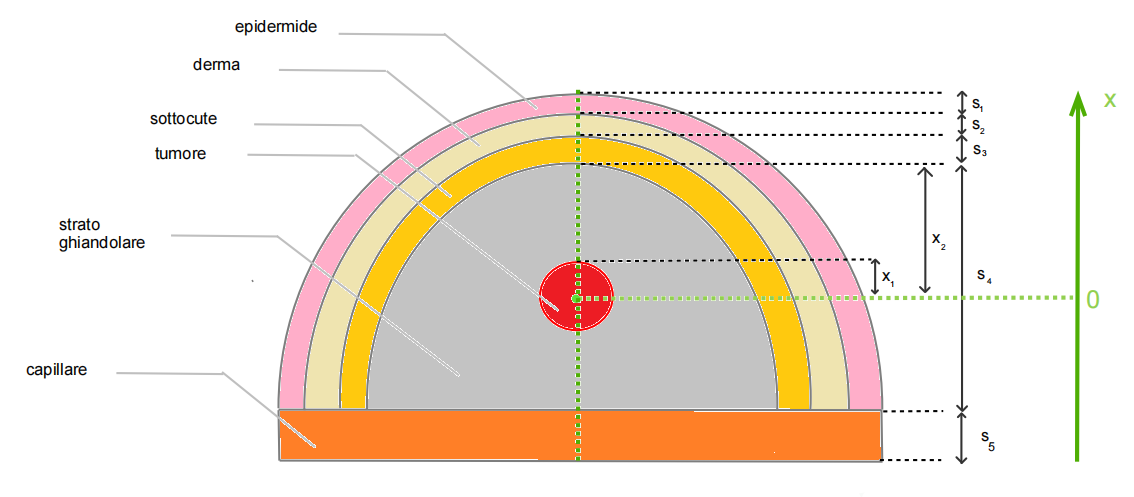
\includegraphics[width=1\textwidth]{Immagini/sistema_1.png} 
    \caption{Schematizzazione del tessuto mammario}
    \label{sistema}
\end{figure}

\vspace{0.1cm}
%\newline
\noindent
L’equazione generale della conduzione può essere scritta come:
\begin{center}
	$\rho c \frac{\partial{T}}{\partial{\theta}}= K  \frac{\partial^2{T}}{\partial{x^2}}+ w_b (T) \rho _b c_b (T_b(\theta)-T) + \Dot{Q} _{met} +\Dot{Q} _{p}$
\end{center}
Considerare la dipendenza dalla temperatura della perfusione sanguigna e delle proprietà elettriche dei tessuti, mentre la conducibilità termica può essere assunta costante.\\\\Di seguito si definiscono le equazioni generalizzate per i singoli nodi caratteristici, supponendo tutte le potenze entranti. Per non appesantire la notazione si suppone che il passo di campionamento nella direzione z e y sia unitario, in modo da trascurarlo durante i calcoli.

%%%%%%%%%%%%%%%%%%%%%%%%%%%%%%%%%%%%%%%%%%%%%%%%%%%%%%%%%%%%%%%%%%
%%%%%%%%%%%%%%%%%%%%%%%%%%%%NODO 1%%%%%%%%%%%%%%%%%%%%%%%%%%%%%%%%

\subsubsection*{Nodo 1}
Il nodo 1 è posto in corrispondenza dell'interfaccia tra l'epidermide e l'ambiente circostante.\\Il bilancio, in questa posizione fornisce:
\begin{center}
	$ \Dot{Q} _{k, i-1} +\Dot{Q} _{c, i}+ \Dot{Q} _{m} +\Dot{Q} _{p}+ w_b (T) \rho _b c_b (T_b(\theta)-T_i ^?)= \frac{\Delta U}{\Delta \theta} $
\end{center}

\vspace{0.1cm}
%\newline
\begin{center}
	$ \frac{k_{ep} A }{\Delta x}(T_{i-1} ^? - T_i ^? ) + h_\infty A (T_{\infty}  - T_i ^? )+ \Dot{Q} _{m} + SAR_i \rho _{ep} \frac{\Delta x}{2}  + w_b (T) \rho _b c_b (T_b(\theta)-T_i ^?) = \rho _{ep} c_{ep} A \frac{\Delta x}{2 \Delta \theta}(T_i ^{t+1} - T_i ^t )$
\end{center}
Dividiamo per $k_{ep}$, per A e moltiplichiamo per $\Delta x$ :
\begin{center}
	$(T_{i-1} ^? - T_i ^? ) + h_\infty \frac{\Delta x }{k_{ep}} (T_{\infty} - T_i ^? )+ \Dot{Q} _{m} \frac{\Delta x }{k_{ep}}+ SAR_i \rho _{ep} \frac{\Delta x^2}{2k_{ep}}  + \frac{ w_b (T) \rho _b c_b \Delta x }{k_{ep}}(T_b(\theta)-T_i ^?) = \rho _{ep} c_{ep}\frac{\Delta x^2}{2 k_{ep} \Delta \theta}(T_i ^{t+1} - T_i ^t )$
\end{center}
\vspace{0.1cm}
\noindent
Definiamo il numero di Biot locale in corrispondenza dell'epidermide:\\
\begin{center}
	$Bi_{ep}= h_\infty \frac{\Delta x }{k_{ep}}$
\end{center}
Definiamo il numero di Fourier in corrispondenza dell'epidermide:
\begin{center}
	$Fo_{ep}= \frac{k_{ep} \Delta \theta}{\rho _{ep} c_{ep} \Delta x^2}$
\end{center}
Sfruttando le costanti appena definite, è possibile riscrive il bilancio come segue:
\begin{center}
	$(T_{i-1} ^? - T_i ^? ) + Bi_{ep} (T_{\infty} - T_i ^? )+ \Dot{Q} _{m} \frac{\Delta x }{k_{ep}}+ SAR_i \rho _{ep} \frac{\Delta x^2}{2k_{ep}}  + \frac{ w_b (T) \rho _b c_b \Delta x }{k_{ep}}(T_b(\theta)-T_i ^?) = \frac{1}{2 Fo_{ep}}(T_i ^{t+1} - T_i ^t )$
\end{center}
Da qui ricaviamo:
\begin{center}
	$T_i ^{t+1}$
 \begin{center}
    \begin{center}
        $\Downarrow$
    \end{center}
 \end{center}
 $T_i ^t + 2 Fo_{ep} \Bigg[ T_{i-1} ^? - T_i ^? \Big(1 + Bi_{ep} +  \frac{ w_b (T) \rho _b c_b \Delta x }{k_{ep}} \Big) + Bi_{ep} T_{\infty} +  \frac{\Delta x }{k_{ep}} \Big(\Dot{Q} _{m} +  SAR_i \rho _{ep} \frac{\Delta x}{2} + w_b (T) \rho _b c_b T_b(\theta)\Big) \Bigg]$
\end{center}


\begin{figure}[H]
    \centering
    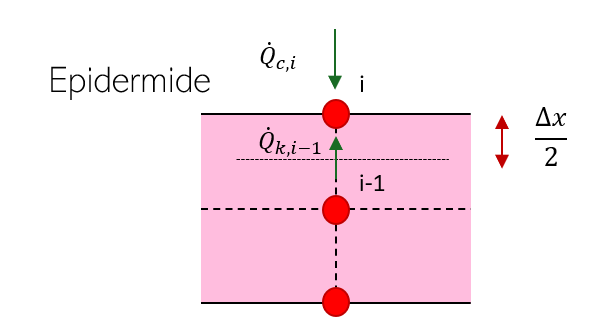
\includegraphics[width=.6\textwidth]{Immagini/Nodi/nodo1.png} 
    \label{nodo1}
\end{figure}


%%%%%%%%%%%%%%%%%%%%%%%%%%%%%%%%%%%%%%%%%%%%%%%%%%%%%%%%%%%%%%%%%%
%%%%%%%%%%%%%%%%%%%%%%%%%%%%NODO 2%%%%%%%%%%%%%%%%%%%%%%%%%%%%%%%%
\subsubsection*{Nodo 2}
Il nodo 2 è posto in corrispondenza in corrispondenza dell'epidermide.\\Il bilancio, in questa posizione fornisce:
\begin{center}
	$ \Dot{Q} _{k, i-1} +\Dot{Q} _{k, i+1}+ \Dot{Q} _{m} +\Dot{Q} _{p}+ w_b (T) \rho _b c_b (T_b(\theta)-T_i ^?)= \frac{\Delta u}{\Delta \theta} $
\end{center}
\vspace{0.15cm}
\begin{center}
	$ \frac{k_{ep} A }{\Delta x}(T_{i-1} ^? - T_i ^? ) + \frac{k_{ep} A }{\Delta x}(T_{i+1} ^? - T_i ^? )+ \Dot{Q} _{m} + SAR_i \rho _{ep} \Delta x  + w_b (T) \rho _b c_b (T_b(\theta)-T_i ^?) = \rho _{ep} c_{ep} A \frac{\Delta x}{ \Delta \theta}(T_i ^{t+1} - T_i ^t )$
\end{center}
\newpage
\noindent
Dividendo per $k_{ep}$, per A e moltiplichiamo per $\Delta x$ otteniamo che:
\begin{center}
	$T_i ^{t+1} $
\end{center}
\begin{center}
	$\Downarrow$
\end{center}
\begin{center}
	$T_i ^t + Fo_{ep} \Bigg[ T_{i-1} ^? + T_{i+1} ^?- T_i ^? \Big(2 + \frac{ w_b (T) \rho _b c_b \Delta x }{k_{ep}} \Big) +  \frac{\Delta x }{k_{ep}} \Big(\Dot{Q} _{m} +  SAR_i \rho _{ep} \Delta x + w_b (T) \rho _b c_b T_b(\theta)\Big) \Bigg]$
\end{center}
\begin{figure}[H]
    \centering
    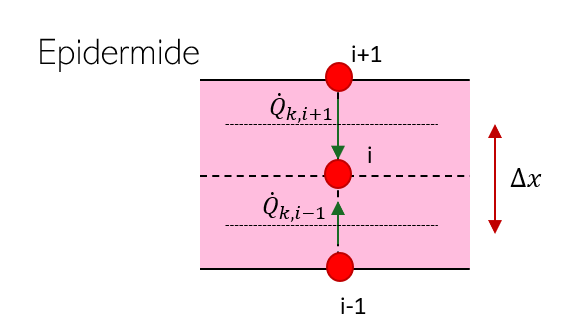
\includegraphics[width=.6\textwidth]{Immagini/Nodi/nodo2.png} 
    \label{nodo2}
\end{figure}


%%%%%%%%%%%%%%%%%%%%%%%%%%%%%%%%%%%%%%%%%%%%%%%%%%%%%%%%%%%%%%%%%%
%%%%%%%%%%%%%%%%%%%%%%%%%%%%NODO 3%%%%%%%%%%%%%%%%%%%%%%%%%%%%%%%%

\subsubsection*{Nodo 3}
Il nodo 3 è posto in corrispondenza dell'interfaccia tra l'epidermide e il derma.
\begin{figure}[H]
    \centering
    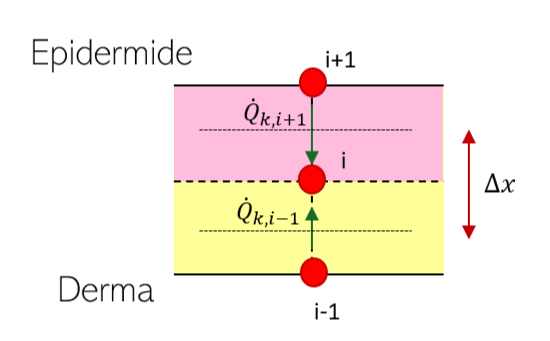
\includegraphics[width=.6\textwidth]{Immagini/Nodi/nodo3.png} 
    \label{nodo3}
\end{figure}
\noindent
Il bilancio, in questa posizione fornisce:
\begin{center}
	$ \Dot{Q} _{k, i-1} +\Dot{Q} _{k, i+1}+ \Dot{Q} _{m} +\Dot{Q} _{p}+ w_b (T) \rho _b c_b (T_b(\theta)-T_i ^?)= \frac{\Delta u}{\Delta \theta} $
\end{center}
Da varie ricerche in letteratura si può ipotizzare che la densità, il calore specifico  e la conducibilità del derma sono le stesse di quella dell'epidermide:
\begin{center}
	$ \frac{k_{ep} A }{\Delta x}(T_{i-1} ^? - T_i ^? ) + \frac{k_{ep} A }{\Delta x}(T_{i+1} ^? - T_i ^? )+ \Dot{Q} _{m} + SAR_i \rho _{ep} \Delta x + w_b (T) \rho _b c_b (T_b(\theta)-T_i ^?) = \rho _{ep} c_{ep} A \frac{\Delta x}{ \Delta \theta}(T_i ^{t+1} - T_i ^t )$
\end{center}
\newpage
\noindent
Dividendo per $k_{ep}$, per A e moltiplichiamo per $\Delta x$ otteniamo che:
\begin{center}
	$T_i ^{t+1} $
\end{center}
\begin{center}
	$\Downarrow$
\end{center}
\begin{center}
	$T_i ^t + Fo_{ep} \Bigg[ T_{i-1} ^? + T_{i+1} ^?- T_i ^? \Big(2 + \frac{ w_b (T) \rho _b c_b \Delta x }{k_{ep}} \Big) +  \frac{\Delta x }{k_{ep}} \Big(\Dot{Q} _{m} +  SAR_i \rho _{ep} \Delta x + w_b (T) \rho _b c_b T_b(\theta)\Big) \Bigg]$
\end{center}

%%%%%%%%%%%%%%%%%%%%%%%%%%%%%%%%%%%%%%%%%%%%%%%%%%%%%%%%%%%%%%%%%%
%%%%%%%%%%%%%%%%%%%%%%%%%%%%NODO 4%%%%%%%%%%%%%%%%%%%%%%%%%%%%%%%%
\subsubsection*{Nodo 4}
Il nodo 4 è posto in corrispondenza del derma.
\begin{figure}[H]
    \centering
    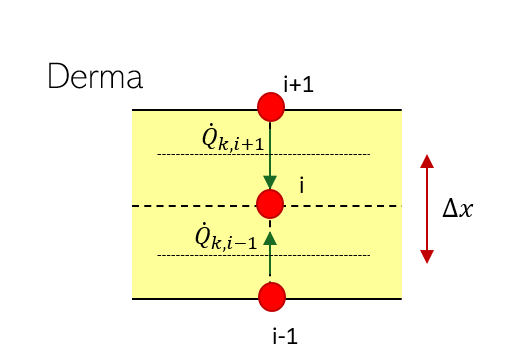
\includegraphics[width=.6\textwidth]{Immagini/Nodi/nodo4.png} 
    \label{nodo4}
\end{figure}
\noindent
Il bilancio, in questa posizione fornisce:
\begin{center}
	$ \Dot{Q} _{k, i-1} +\Dot{Q} _{k, i+1}+ \Dot{Q} _{m} +\Dot{Q} _{p}+ w_b (T) \rho _b c_b (T_b(\theta)-T_i ^?)= \frac{\Delta u}{\Delta \theta} $
\end{center}
Da varie ricerche in letteratura si può ipotizzare che la densità, il calore specifico  e la conducibilità del derma sono le stesse di quella dell'epidermide:
\begin{center}
	$ \frac{k_{ep} A }{\Delta x}(T_{i-1} ^? - T_i ^? ) + \frac{k_{ep} A }{\Delta x}(T_{i+1} ^? - T_i ^? )+ \Dot{Q} _{m} + SAR_i \rho _{ep} \Delta x  + w_b (T) \rho _b c_b (T_b(\theta)-T_i ^?) = \rho _{ep} c_{ep} A \frac{\Delta x}{ \Delta \theta}(T_i ^{t+1} - T_i ^t )$
\end{center}

\noindent
Dividendo per $k_{ep}$, per A e moltiplichiamo per $\Delta x$ otteniamo che:
\begin{center}
	$T_i ^{t+1} $
\end{center}
\begin{center}
	$\Downarrow$
\end{center}
\begin{center}
	$T_i ^t + Fo_{ep} \Bigg[ T_{i-1} ^? + T_{i+1} ^?- T_i ^? \Big(2 + \frac{ w_b (T) \rho _b c_b \Delta x }{k_{ep}} \Big) +  \frac{\Delta x }{k_{ep}} \Big(\Dot{Q} _{m} +  SAR_i \rho _{ep} \Delta x + w_b (T) \rho _b c_b T_b(\theta)\Big) \Bigg]$
\end{center}

%%%%%%%%%%%%%%%%%%%%%%%%%%%%%%%%%%%%%%%%%%%%%%%%%%%%%%%%%%%%%%%%%%
%%%%%%%%%%%%%%%%%%%%%%%%%%%%NODO 5%%%%%%%%%%%%%%%%%%%%%%%%%%%%%%%%

\subsubsection*{Nodo 5}

Il nodo 5 è posto a cavallo dell'interfaccia tra derma e sottocute.
\begin{figure}[H]
    \centering
    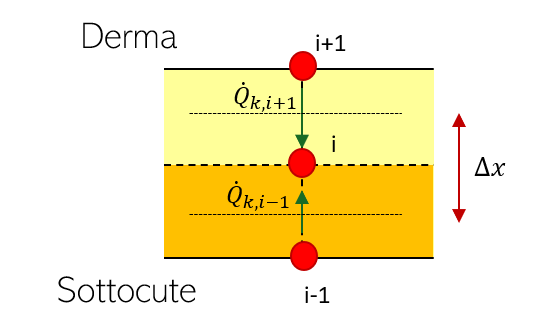
\includegraphics[width=.6\textwidth]{Immagini/Nodi/nodo5.png} 
    \label{nodo5}
\end{figure}
\noindent
Il bilancio, in questa posizione fornisce:
\begin{center}
	$ \Dot{Q} _{k, i-1} +\Dot{Q} _{k, i+1}+ \Dot{Q} _{m} +\Dot{Q} _{p}+ w_b (T) \rho _b c_b (T_b(\theta)-T_i ^?)= \frac{\Delta u}{\Delta \theta} $
\end{center}
Da varie ricerche in letteratura si può ipotizzare che la densità, il calore specifico  e la conducibilità della sottocute sono le stesse di quella dell'epidermide:
\begin{center}
	$ \frac{k_{ep} A }{\Delta x}(T_{i-1} ^? - T_i ^? ) + \frac{k_{ep} A }{\Delta x}(T_{i+1} ^? - T_i ^? )+ \Dot{Q} _{m} + SAR_i \rho _{ep} \Delta x  + w_b (T) \rho _b c_b (T_b(\theta)-T_i ^?) = \rho _{ep} c_{ep} A \frac{\Delta x}{ \Delta \theta}(T_i ^{t+1} - T_i ^t )$
\end{center}

\noindent
Dividendo per $k_{ep}$, per A e moltiplichiamo per $\Delta x$ otteniamo che:
\begin{center}
	$T_i ^{t+1} $
\end{center}
\begin{center}
	$\Downarrow$
\end{center}
\begin{center}
	$T_i ^t + Fo_{ep} \Bigg[ T_{i-1} ^? + T_{i+1} ^?- T_i ^? \Big(2 + \frac{ w_b (T) \rho _b c_b \Delta x }{k_{ep}} \Big) +  \frac{\Delta x }{k_{ep}} \Big(\Dot{Q} _{m} +  SAR_i \rho _{ep} \Delta x + w_b (T) \rho _b c_b T_b(\theta)\Big) \Bigg]$
\end{center}

%%%%%%%%%%%%%%%%%%%%%%%%%%%%%%%%%%%%%%%%%%%%%%%%%%%%%%%%%%%%%%%%%%
%%%%%%%%%%%%%%%%%%%%%%%%%%%%NODO 6%%%%%%%%%%%%%%%%%%%%%%%%%%%%%%%%
\subsubsection*{Nodo 6}

Il nodo 6 è posto in corrispondenza della sottocute.\\
Il bilancio, in questa posizione fornisce:
\vspace{0.5cm}
\begin{center}
	$ \Dot{Q} _{k, i-1} +\Dot{Q} _{k, i+1}+ \Dot{Q} _{m} +\Dot{Q} _{p}+ w_b (T) \rho _b c_b (T_b(\theta)-T_i ^?)= \frac{\Delta u}{\Delta \theta} $
\end{center}
\vspace{0.5cm}
Da varie ricerche in letteratura si può ipotizzare che la densità, il calore specifico  e la conducibilità della sottocute sono le stesse di quella dell'epidermide:
\vspace{0.5cm}
\begin{center}
	$ \frac{k_{ep} A }{\Delta x}(T_{i-1} ^? - T_i ^? ) + \frac{k_{ep} A }{\Delta x}(T_{i+1} ^? - T_i ^? )+ \Dot{Q} _{m} + SAR_i \rho _{ep} \Delta x  + w_b (T) \rho _b c_b (T_b(\theta)-T_i ^?) = \rho _{ep} c_{ep} A \frac{\Delta x}{ \Delta \theta}(T_i ^{t+1} - T_i ^t )$
\end{center}
\begin{figure}[H]
    \centering
    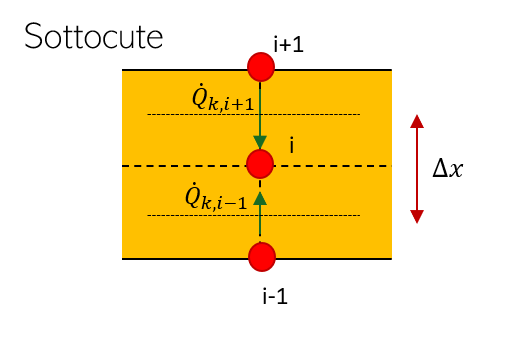
\includegraphics[width=.6\textwidth]{Immagini/Nodi/nodo6.png} 
    \label{nodo2}
\end{figure}
\noindent

\noindent
Dividendo per $k_{ep}$, per A e moltiplichiamo per $\Delta x$ otteniamo che:
\begin{center}
	$T_i ^{t+1} $
\end{center}
\begin{center}
	$\Downarrow$
\end{center}
\begin{center}
	$T_i ^t + Fo_{ep} \Bigg[ T_{i-1} ^? + T_{i+1} ^?- T_i ^? \Big(2 + \frac{ w_b (T) \rho _b c_b \Delta x }{k_{ep}} \Big) +  \frac{\Delta x }{k_{ep}} \Big(\Dot{Q} _{m} +  SAR_i \rho _{ep} \Delta x + w_b (T) \rho _b c_b T_b(\theta)\Big) \Bigg]$
\end{center}
%%%%%%%%%%%%%%%%%%%%%%%%%%%%%%%%%%%%%%%%%%%%%%%%%%%%%%%%%%%%%%%%%%
%%%%%%%%%%%%%%%%%%%%%%%%%%%%NODO 7%%%%%%%%%%%%%%%%%%%%%%%%%%%%%%%%
\subsubsection*{Nodo 7}
Il nodo 7 è posto in corrispondenza dell'interfaccia tra sottocute e strati ghiandolare.
\begin{figure}[H]
    \centering
    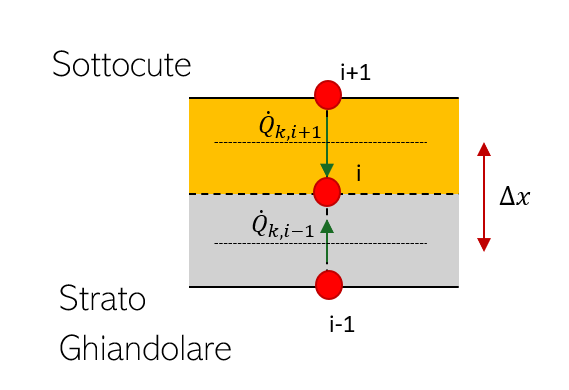
\includegraphics[width=.6\textwidth]{Immagini/Nodi/nodo7.png} 
    \label{nodo7}
\end{figure}
\noindent
Il bilancio, in questa posizione fornisce:
\begin{center}
	$ \Dot{Q} _{k, i-1} +\Dot{Q} _{k, i+1}+ \Dot{Q} _{m} +\Dot{Q} _{p}+ w_b (T) \rho _b c_b (T_b(\theta)-T_i ^?)= \frac{\Delta u}{\Delta \theta} $
\end{center}
\vspace{0.15cm}
\begin{center}
	$ \frac{k_{ep} A }{\Delta x}(T_{i+1} ^? - T_i ^? ) + \frac{k_g A }{\Delta x}(T_{i-1} ^? - T_i ^? )+ \Dot{Q} _{m} + SAR_i \frac{\rho _{ep} + \rho _g}{2} \Delta x + w_b (T) \rho _b c_b (T_b(\theta)-T_i ^?) = \frac{\Delta x}{ 2 \Delta \theta}(T_i ^{t+1} - T_i ^t ) (\rho _{ep} c_{ep} + \rho _{g} c_{g} )$
\end{center}
Definiamo il numero di Fourier in corrispondenza dello strato ghiandolare:
\begin{center}
	$Fo_{g}= \frac{k_{g} \Delta \theta}{\rho _{g} c_{g} \Delta x^2}$
\end{center}
Un ulteriore parametro da introdurre per semplificare la scrittura equivalente un il numero di Fourier equivalente che tiene conto, contemporaneamente della sottocute e dello strato ghiandolare:
\begin{center}
	$\frac{1}{Fo_{eg}}= \frac{1}{Fo_{ep}k_g}+ \frac{1}{Fo_{g}k_{ep}}$
\end{center}
Da queste definizione si ottiene:
\begin{center}
	$T_i ^{t+1} $
\end{center}
\begin{center}
	$\Downarrow$
\end{center}
\begin{center}
	$T_i ^t + Fo_{eg} \Bigg[ 2\frac{T_{i-1} ^?}{k_ep} + 2\frac{T_{i+1} ^?}{k_{g}}- 2T_i ^? \Big(\frac{1}{k_g} + \frac{1}{k_{ep}}+ \frac{ w_b (T) \rho _b c_b \Delta x }{k_{ep}k_g} \Big) +  \frac{\Delta x }{k_{ep}k_g} \Big(2\Dot{Q} _{m} +  SAR_i (\rho _{ep}+ \rho _g) \Delta x + 2w_b (T) \rho _b c_b T_b(\theta)\Big) \Bigg]$
\end{center}



%%%%%%%%%%%%%%%%%%%%%%%%%%%%%%%%%%%%%%%%%%%%%%%%%%%%%%%%%%%%%%%%%%
%%%%%%%%%%%%%%%%%%%%%%%%%%%%NODO 8%%%%%%%%%%%%%%%%%%%%%%%%%%%%%%%%
\subsubsection*{Nodo 8}
Il nodo 8 è posto in corrispondenza dello strato ghiandolare.\\
In questa posizione il nodo i+1 può assumere due possibili configurazioni differenti:
\begin{enumerate}
    \item in corrispondenza dell'interfaccia tra sottocute e strato ghiandolare;
    \item in corrispondenza dello strato ghiandolare.
\end{enumerate}
Di seguito vengono analizzate le due casistiche.
\begin{description}
    \item[I CASO: i+1 all'interfaccia sottocute-strato ghiandolare]
    \begin{figure}[H]
    \centering
    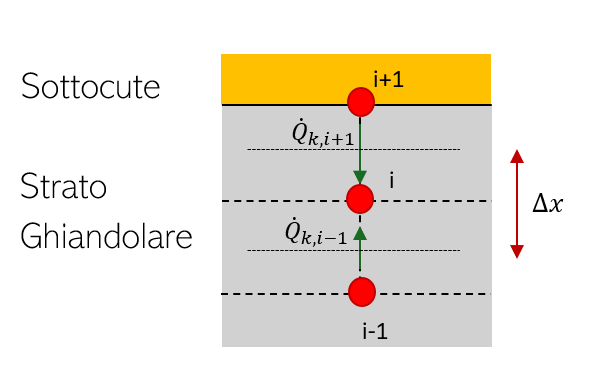
\includegraphics[width=.6\textwidth]{Immagini/Nodi/nodo8.1.png} 
    \caption{i+1 all'interfaccia sottocute-strato ghiandolare}
    \label{nodo8.1}
\end{figure}
\noindent
\newpage
Il bilancio, in questa posizione fornisce:
\begin{center}
	$ \Dot{Q} _{k, i-1} +\Dot{Q} _{k, i+1}+ \Dot{Q} _{m} +\Dot{Q} _{p}+ w_b (T) \rho _b c_b (T_b(\theta)-T_i ^?)= \frac{\Delta u}{\Delta \theta} $
\end{center}
\vspace{0.15cm}
\begin{center}
	$ \frac{k_g+ k_{ep}}{2} \cdot\frac{ A }{\Delta x}(T_{i+1} ^? - T_i ^? ) + \frac{k_g A }{\Delta x}(T_{i-1} ^? - T_i ^? )+ \Dot{Q} _{m} + SAR_i\rho _g \Delta x + w_b (T) \rho _b c_b (T_b(\theta)-T_i ^?) = \rho _{g} c_{g} A \frac{\Delta x}{ \Delta \theta}(T_i ^{t+1} - T_i ^t ) $
\end{center}
Con le opportune semplificazioni, si ottiene:
\begin{center}
	$T_i ^{t+1} $
\end{center}
\begin{center}
	$\Downarrow$
\end{center}
\begin{center}
	$T_i ^t + Fo_{g} \Bigg[ T_{i+1} ^? (\frac{k_g+ k_{ep}}{2 k_g}) + T_{i-1} ^?- T_i ^? \Big(\frac{k_g+ k_{ep}}{2 k_g} + 1 + \frac{ w_b (T) \rho _b c_b \Delta x }{k_{g}} \Big) + \frac{\Delta x }{k_{g}} \Big(\Dot{Q} _{m} +  SAR_i \rho _{g} \Delta x + w_b (T) \rho _b c_b T_b(\theta)\Big) \Bigg]$
\end{center}


\item[II CASO: i+1 nella sottocute]

     \begin{figure}[H]
    \centering
    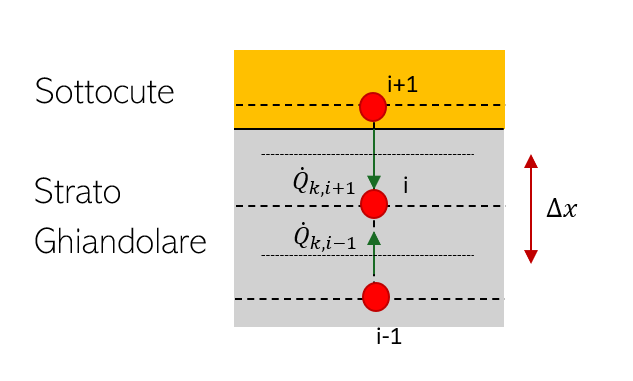
\includegraphics[width=.6\textwidth]{Immagini/Nodi/nodo8.2.png} 
    \label{nodo8.2}
    \caption{i+1 nella sottocute}
\end{figure}
\end{description}
Il bilancio, in questa posizione fornisce:
\begin{center}
	$ \Dot{Q} _{k, i-1} +\Dot{Q} _{k, i+1}+ \Dot{Q} _{m} +\Dot{Q} _{p}+ w_b (T) \rho _b c_b (T_b(\theta)-T_i ^?)= \frac{\Delta u}{\Delta \theta} $
\end{center}
\vspace{0.15cm}
\begin{center}
	$ \frac{k_{ep} A }{\Delta x}(T_{i+1} ^? - T_i ^? ) + \frac{k_g A }{\Delta x}(T_{i-1} ^? - T_i ^? )+ \Dot{Q} _{m} + SAR_i\rho _g \Delta x + w_b (T) \rho _b c_b (T_b(\theta)-T_i ^?) = \rho _{g} c_{g} A \frac{\Delta x}{ \Delta \theta}(T_i ^{t+1} - T_i ^t ) $
\end{center}
Con le opportune semplificazioni, si ottiene:
\begin{center}
	$T_i ^{t+1} $
\end{center}
\begin{center}
	$\Downarrow$
\end{center}
\begin{center}
	$T_i ^t + Fo_{g} \Bigg[ T_{i+1} ^? \frac{k_{ep}}{k_{g}} + T_{i-1} ^?- T_i ^? \Big(\frac{k_{ep}}{k_{g}} + 1 + \frac{ w_b (T) \rho _b c_b \Delta x }{k_{g}} \Big) + \frac{\Delta x }{k_{g}} \Big(\Dot{Q} _{m} +  SAR_i \rho _{g} \Delta x + w_b (T) \rho _b c_b T_b(\theta)\Big) \Bigg]$
\end{center}


%%%%%%%%%%%%%%%%%%%%%%%%%%%%%%%%%%%%%%%%%%%%%%%%%%%%%%%%%%%%%%%%%%
%%%%%%%%%%%%%%%%%%%%%%%%%%%%NODO 9%%%%%%%%%%%%%%%%%%%%%%%%%%%%%%%%
\subsubsection*{Nodo 9}
Il nodo 9 è posto in corrispondenza dello strato ghiandolare.\\
\begin{figure}[H]
    \centering
    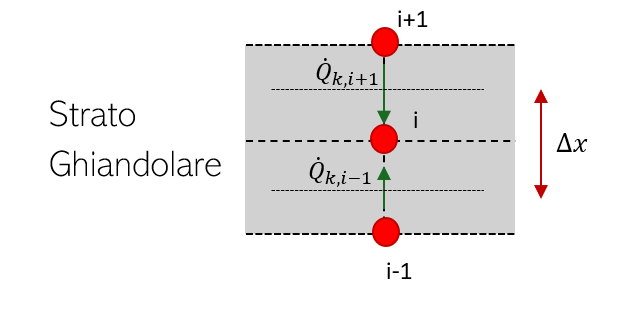
\includegraphics[width=.6\textwidth]{Immagini/Nodi/nodo9.png} 
    \label{nodo9}
\end{figure}
\noindent
Il bilancio, in questa posizione fornisce:
\begin{center}
	$ \Dot{Q} _{k, i-1} +\Dot{Q} _{k, i+1}+ \Dot{Q} _{m} +\Dot{Q} _{p}+ w_b (T) \rho _b c_b (T_b(\theta)-T_i ^?)= \frac{\Delta u}{\Delta \theta} $
\end{center}
\vspace{0.15cm}
\begin{center}
	$ \frac{k_{g} A }{\Delta x}(T_{i+1} ^? - T_i ^? ) + \frac{k_g A }{\Delta x}(T_{i-1} ^? - T_i ^? )+ \Dot{Q} _{m} + SAR_i\rho _g \Delta x + w_b (T) \rho _b c_b (T_b(\theta)-T_i ^?) = \rho _{g} c_{g} A \frac{\Delta x}{ \Delta \theta}(T_i ^{t+1} - T_i ^t ) $
\end{center}
Con le opportune semplificazioni, si ottiene:
\begin{center}
	$T_i ^{t+1} $
\end{center}
\begin{center}
	$\Downarrow$
\end{center}
\begin{center}
	$T_i ^t + Fo_{g} \Bigg[ T_{i-1} ^? + T_{i+1} ^?- T_i ^? \Big(2 + \frac{ w_b (T) \rho _b c_b \Delta x }{k_{g}} \Big) + \frac{\Delta x }{k_{g}} \Big(\Dot{Q} _{m} +  SAR_i \rho _{g} \Delta x + w_b (T) \rho _b c_b T_b(\theta)\Big) \Bigg]$
\end{center}



%%%%%%%%%%%%%%%%%%%%%%%%%%%%%%%%%%%%%%%%%%%%%%%%%%%%%%%%%%%%%%%%%%
%%%%%%%%%%%%%%%%%%%%%%%%%%%%NODO 10%%%%%%%%%%%%%%%%%%%%%%%%%%%%%%%%



\subsubsection*{Nodo 10}
Il nodo 10 è posto in corrispondenza dello strato ghiandolare.\\
In questa posizione il nodo i-1 può avere due configurazioni differenti:
\begin{enumerate}
    \item in corrispondenza dell'interfaccia tra strato ghiandolare e tumore;
    \item in corrispondenza del tumore.
\end{enumerate}
Di seguito vengono analizzate le due casistiche.
\begin{description}
    \item[I CASO: i-1 all'interfaccia strato ghiandolare-tumore]
    \begin{figure}[H]
    \centering
    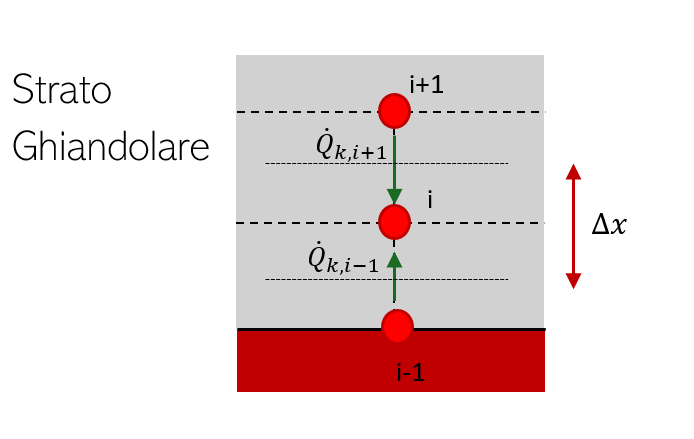
\includegraphics[width=.6\textwidth]{Immagini/Nodi/nodo11.1.png} 
    \caption{i-1 all'interfaccia strato ghiandolare-tumore}
    \label{nodo10.1}
\end{figure}
\noindent
\newline
\noindent
Il bilancio, in questa posizione fornisce:
\begin{center}
	$ \Dot{Q} _{k, i-1} +\Dot{Q} _{k, i+1}+ \Dot{Q} _{m} +\Dot{Q} _{p}+ w_b (T) \rho _b c_b (T_b(\theta)-T_i ^?)= \frac{\Delta u}{\Delta \theta} $
\end{center}
\vspace{0.15cm}
\begin{center}
	$ \frac{k_g+ k_{t}}{2} \cdot\frac{ A }{\Delta x}(T_{i-1} ^? - T_i ^? ) + \frac{k_g A }{\Delta x}(T_{i+1} ^? - T_i ^? )+ \Dot{Q} _{m} + SAR_i\rho _g \Delta x + w_b (T) \rho _b c_b (T_b(\theta)-T_i ^?) = \rho _{g} c_{g} A \frac{\Delta x}{ \Delta \theta}(T_i ^{t+1} - T_i ^t ) $
\end{center}
Con le opportune semplificazioni, si ottiene:
\begin{center}
	$T_i ^{t+1} $
\end{center}
\begin{center}
	$\Downarrow$
\end{center}
\begin{center}
	$T_i ^t + Fo_{g} \Bigg[ T_{i-1} ^? (\frac{k_g+ k_{t}}{2 k_g}) + T_{i+1} ^?- T_i ^? \Big(\frac{k_g+ k_{t}}{2k_g} + 1 + \frac{ w_b (T) \rho _b c_b \Delta x }{k_{g}} \Big) + \frac{\Delta x }{k_{g}} \Big(\Dot{Q} _{m} +  SAR_i \rho _{g} \Delta x + w_b (T) \rho _b c_b T_b(\theta)\Big) \Bigg]$
\end{center}


\item[II CASO: i-1 nel tumore]

     \begin{figure}[H]
    \centering
    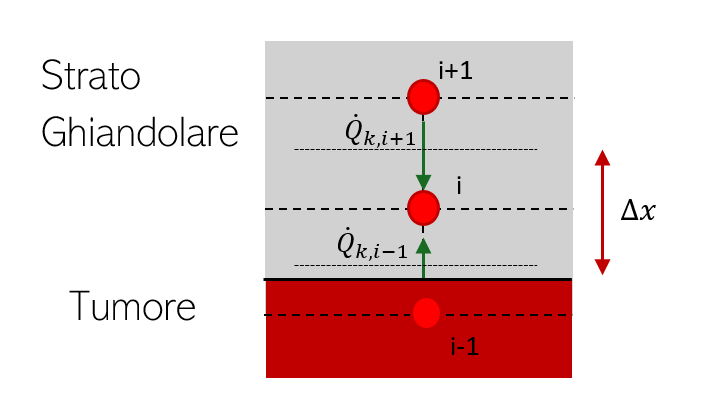
\includegraphics[width=.6\textwidth]{Immagini/Nodi/nodo11.2.png} 
    \caption{i-1 nel tumore}
    \label{nodo8.2}
\end{figure}
\end{description}
Il bilancio, in questa posizione fornisce:
\begin{center}
	$ \Dot{Q} _{k, i-1} +\Dot{Q} _{k, i+1}+ \Dot{Q} _{m} +\Dot{Q} _{p}+ w_b (T) \rho _b c_b (T_b(\theta)-T_i ^?)= \frac{\Delta u}{\Delta \theta} $
\end{center}
\vspace{0.15cm}
\begin{center}
	$ \frac{k_{g} A }{\Delta x}(T_{i+1} ^? - T_i ^? ) + \frac{k_t A }{\Delta x}(T_{i-1} ^? - T_i ^? )+ \Dot{Q} _{m} + SAR_i\rho _g \Delta x + w_b (T) \rho _b c_b (T_b(\theta)-T_i ^?) = \rho _{g} c_{g} A \frac{\Delta x}{ \Delta \theta}(T_i ^{t+1} - T_i ^t ) $
\end{center}
Con le opportune semplificazioni, si ottiene:
\begin{center}
	$T_i ^{t+1} $
\end{center}
\begin{center}
	$\Downarrow$
\end{center}
\begin{center}
	$T_i ^t + Fo_{g} \Bigg[ T_{i-1} ^? \frac{k_{t}}{k_g} + T_{i+1} ^?- T_i ^? \Big(\frac{k_{t}}{k_g} + 1 + \frac{ w_b (T) \rho _b c_b \Delta x }{k_{g}} \Big) + \frac{\Delta x }{k_{g}} \Big(\Dot{Q} _{m} +  SAR_i \rho _{g} \Delta x + w_b (T) \rho _b c_b T_b(\theta)\Big) \Bigg]$
\end{center}
%%%%%%%%%%%%%%%%%%%%%%%%%%%%%%%%%%%%%%%%%%%%%%%%%%%%%%%%%%%%%%%%%%
%%%%%%%%%%%%%%%%%%%%%%%%%%%%NODO 11%%%%%%%%%%%%%%%%%%%%%%%%%%%%%%%%
\subsubsection*{Nodo 11}
Il nodo 11 è posto in corrispondenza dell'interfaccia tra strato ghiandolare e tumore.
\begin{figure}[H]
    \centering
    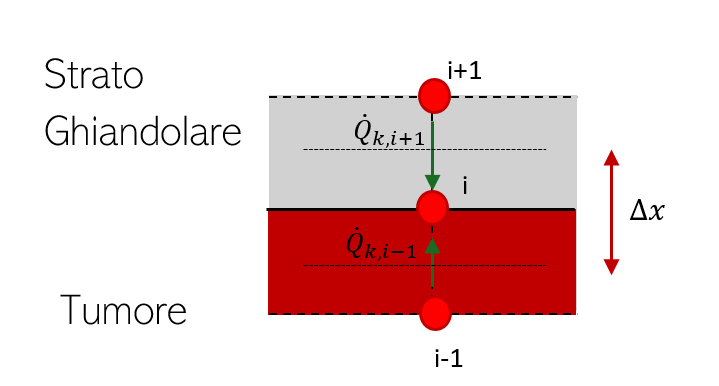
\includegraphics[width=.6\textwidth]{Immagini/Nodi/nodo10.png} 
    \label{nodo11}
\end{figure}
\noindent
Il bilancio, in questa posizione fornisce:
\begin{center}
	$ \Dot{Q} _{k, i-1} +\Dot{Q} _{k, i+1}+ \Dot{Q} _{m} +\Dot{Q} _{p}+ w_b (T) \rho _b c_b (T_b(\theta)-T_i ^?)= \frac{\Delta u}{\Delta \theta} $
\end{center}
\vspace{0.15cm}
\begin{center}
	$ \frac{k_{g} A }{\Delta x}(T_{i+1} ^? - T_i ^? ) + \frac{k_t A }{\Delta x}(T_{i-1} ^? - T_i ^? )+ \Dot{Q} _{m} + SAR_i \frac{\rho _{g} + \rho _t}{2} \Delta x + w_b (T) \rho _b c_b (T_b(\theta)-T_i ^?) = \frac{\Delta x}{ 2 \Delta \theta}(T_i ^{t+1} - T_i ^t ) (\rho _{g} c_{g} + \rho _{t} c_{t} )$
\end{center}
Definiamo il numero di Fourier in corrispondenza dello strato ghiandolare:
\begin{center}
	$Fo_{t}= \frac{k_{t} \Delta \theta}{\rho _{t} c_{t} \Delta x^2}$
\end{center}
Un ulteriore parametro da introdurre per semplificare la scrittura equivalente un il numero di Fourier equivalente che tiene conto, contemporaneamente della sottocute e dello strato ghiandolare:
\begin{center}
	$\frac{1}{Fo_{gt}}= \frac{1}{Fo_{t}k_g}+ \frac{1}{Fo_{g}k_{t}}$
\end{center}
Da queste definizione si ottiene:
\begin{center}
	$T_i ^{t+1} $
\end{center}
\begin{center}
	$\Downarrow$
\end{center}
\begin{center}
	$T_i ^t + Fo_{gt} \Bigg[ 2\frac{T_{i+1} ^?}{k_t} + 2\frac{T_{i-1} ^?}{k_{g}}- 2T_i ^? \Big(\frac{1}{k_t} + \frac{1}{k_{g}}+ \frac{ w_b (T) \rho _b c_b \Delta x }{k_{t}k_g} \Big) +  \frac{\Delta x }{k_{t}k_g} \Big(2\Dot{Q} _{m} +  SAR_i (\rho _{t}+ \rho _g) \Delta x + 2w_b (T) \rho _b c_b T_b(\theta)\Big) \Bigg]$
\end{center}


%%%%%%%%%%%%%%%%%%%%%%%%%%%%%%%%%%%%%%%%%%%%%%%%%%%%%%%%%%%%%%%%%%
%%%%%%%%%%%%%%%%%%%%%%%%%%%%NODO 12%%%%%%%%%%%%%%%%%%%%%%%%%%%%%%%%
\subsubsection*{Nodo 12}
Il nodo 12 è posto in corrispondenza del tumore.\\
In questa posizione il nodo i+1 può stare in due configurazioni differenti:
\begin{enumerate}
    \item in corrispondenza dello strato ghiandolare;
    \item in corrispondenza dell'interfaccia tra strato ghiandolare e tumore.
\end{enumerate}
Di seguito vengono analizzate le due casistiche.
\begin{description}
    

\item[I CASO: i+1 nello strato ghiandolare]

     \begin{figure}[H]
    \centering
    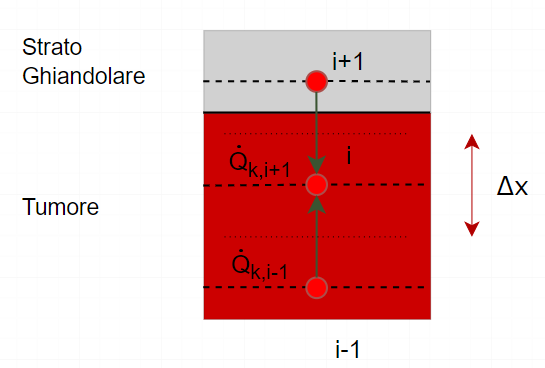
\includegraphics[width=.6\textwidth]{Immagini/Nodi/nodo12.1.png} 
    \label{nodo12.1}
\end{figure}

\noindent
\\Il bilancio, in questa posizione fornisce:
\begin{center}
	$ \Dot{Q} _{k, i-1} +\Dot{Q} _{k, i+1}+ \Dot{Q} _{m} +\Dot{Q} _{p}+ w_b (T) \rho _b c_b (T_b(\theta)-T_i ^?)= \frac{\Delta U}{\Delta \theta} $
\end{center}
Con le opportune semplificazioni, si ottiene:
\begin{center}
	$T_i ^{t+1} $
\end{center}
\begin{center}
	$\Downarrow$
\end{center}
\begin{center}
	$T_i ^t + Fo_{t} \Bigg[ T_{i+1} ^? (\frac{k_{g}}{k_t}) + T_{i-1} ^?- T_i ^? \Big(\frac{k_{g}}{k_t} + 1 + \frac{ w_b (T) \rho _b c_b \Delta x }{k_{t}} \Big) + \frac{\Delta x }{k_{t}} \Big(\Dot{Q} _{m} +  SAR_i \rho _{t} \Delta x + w_b (T) \rho _b c_b T_b(\theta)\Big) \Bigg]$
\end{center}

\item[II CASO: i+1 all'interfaccia strato ghiandolare -tumore]
    \begin{figure}[H]
    \centering
    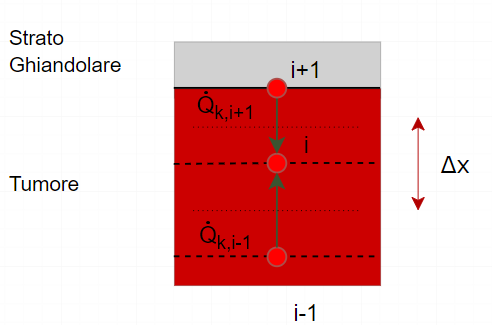
\includegraphics[width=.6\textwidth]{Immagini/Nodi/nodo12.2.png} 
    \label{nodo12}
\end{figure}
\end{description}
\noindent
Il bilancio, in questa posizione fornisce:
\begin{center}
	$ \Dot{Q} _{k, i-1} +\Dot{Q} _{k, i+1}+ \Dot{Q} _{m} +\Dot{Q} _{p}+ w_b (T) \rho _b c_b (T_b(\theta)-T_i ^?)= \frac{\Delta U}{\Delta \theta} $
\end{center}
Con le opportune semplificazioni, si ottiene:
\begin{center}
	$T_i ^{t+1} $
\end{center}
\begin{center}
	$\Downarrow$
\end{center}
\begin{center}
	$T_i ^t + Fo_{t} \Bigg[ T_{i+1} ^? (\frac{k_g+ k_{t}}{2 \: k_t}) + T_{i-1} ^?- T_i ^? \Big(\frac{k_g+ k_{t}}{2 \: k_t} + 1 + \frac{ w_b (T) \rho _b c_b \Delta x }{k_{t}} \Big) + \frac{\Delta x }{k_{t}} \Big(\Dot{Q} _{m} +  SAR_i \rho _{t} \Delta x + w_b (T) \rho _b c_b T_b(\theta)\Big) \Bigg]$
\end{center}

%%%%%%%%%%%%%%%%%%%%%%%%%%%%%%%%%%%%%%%%%%%%%%%%%%%%%%%%%%%%%%%%%%
%%%%%%%%%%%%%%%%%%%%%%%%%%%%NODO 13%%%%%%%%%%%%%%%%%%%%%%%%%%%%%%%%
\subsubsection*{Nodo 13}
Il nodo 13 è posto in corrispondenza del tumore.\\
\begin{figure}[H]
    \centering
    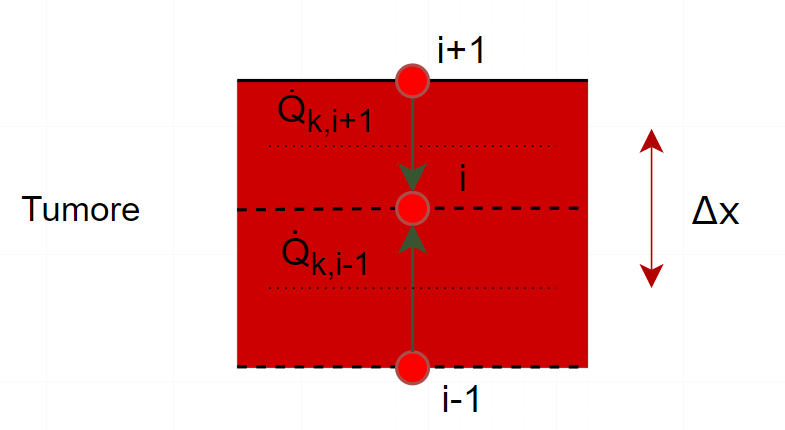
\includegraphics[width=.6\textwidth]{Immagini/Nodi/nodo13.png} 
    \label{nodo13}
\end{figure}
\noindent
Il bilancio, in questa posizione fornisce:
\begin{center}
	$ \Dot{Q} _{k, i-1} +\Dot{Q} _{k, i+1}+ \Dot{Q} _{m} +\Dot{Q} _{p}+ w_b (T) \rho _b c_b (T_b(\theta)-T_i ^?)= \frac{\Delta u}{\Delta \theta} $
\end{center}
Con le opportune semplificazioni, si ottiene:
\begin{center}
	$T_i ^{t+1} $
\end{center}
\begin{center}
	$\Downarrow$
\end{center}
\begin{center}
	$T_i ^t + Fo_{t} \Bigg[ T_{i-1} ^? + T_{i+1} ^?- T_i ^? \Big(2 + \frac{ w_b (T) \rho _b c_b \Delta x }{k_{t}} \Big) + \frac{\Delta x }{k_{t}} \Big(\Dot{Q} _{m} +  SAR_i \rho _{t} \Delta x + w_b (T) \rho _b c_b T_b(\theta)\Big) \Bigg]$
\end{center}

%%%%%%%%%%%%%%%%%%%%%%%%%%%%%%%%%%%%%%%%%%%%%%%%%%%%%%%%%%%%%%%%%%
%%%%%%%%%%%%%%%%%%%%%%%%%%%%NODO 14%%%%%%%%%%%%%%%%%%%%%%%%%%%%%%%%



\subsubsection*{Nodo 14}
Il nodo 14 è posto in corrispondenza del tumore.\\
In questa posizione il nodo i-1 può avere due configurazioni differenti:
\begin{enumerate}
    \item in corrispondenza dell'interfaccia tra tumore e strato ghiandolare;
    \item in corrispondenza dello strato ghiandolare.
\end{enumerate}
Di seguito vengono analizzate le due casistiche.
\begin{description}
    \item[I CASO: i-1 all'interfaccia tumore - strato ghiandolare]
    \begin{figure}[H]
    \centering
    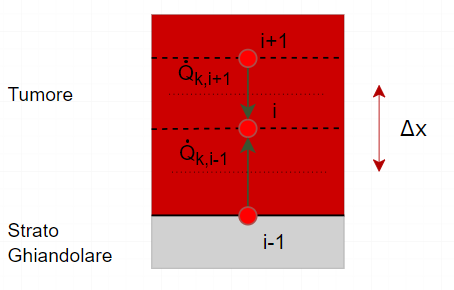
\includegraphics[width=.6\textwidth]{Immagini/Nodi/nodo14.1.png} 
    \label{nodo14}
\end{figure}
\noindent
Il bilancio, in questa posizione fornisce:
\begin{center}
	$ \Dot{Q} _{k, i-1} +\Dot{Q} _{k, i+1}+ \Dot{Q} _{m} +\Dot{Q} _{p}+ w_b (T) \rho _b c_b (T_b(\theta)-T_i ^?)= \frac{\Delta U}{\Delta \theta} $
\end{center}
Con le opportune semplificazioni, si ottiene:
\begin{center}
	$T_i ^{t+1} $
\end{center}
\begin{center}
	$\Downarrow$
\end{center}
\begin{center}
	$T_i ^t + Fo_{t} \Bigg[ T_{i-1} ^? (\frac{k_g+ k_{t}}{2 \: k_t}) + T_{i+1} ^?- T_i ^? \Big(\frac{k_g+ k_{t}}{2 \: k_t} + 1 + \frac{ w_b (T) \rho _b c_b \Delta x }{k_{t}} \Big) + \frac{\Delta x }{k_{t}} \Big(\Dot{Q} _{m} +  SAR_i \rho _{t} \Delta x + w_b (T) \rho _b c_b T_b(\theta)\Big) \Bigg]$
\end{center}


\item[II CASO: i-1 nello strato ghiandolare]

     \begin{figure}[H]
    \centering
    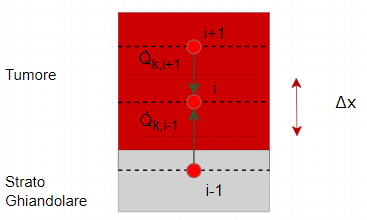
\includegraphics[width=.6\textwidth]{Immagini/Nodi/nodo14.2.png} 
    \label{nodo2}
\end{figure}
\end{description}
Il bilancio, in questa posizione fornisce:
\begin{center}
	$ \Dot{Q} _{k, i-1} +\Dot{Q} _{k, i+1}+ \Dot{Q} _{m} +\Dot{Q} _{p}+ w_b (T) \rho _b c_b (T_b(\theta)-T_i ^?)= \frac{\Delta U}{\Delta \theta} $
\end{center}
Con le opportune semplificazioni, si ottiene:
\begin{center}
	$T_i ^{t+1} $
\end{center}
\begin{center}
	$\Downarrow$
\end{center}
\begin{center}
	$T_i ^t + Fo_{t} \Bigg[ T_{i-1} ^? (\frac{k_{g}}{k_t}) + T_{i+1} ^?- T_i ^? \Big(\frac{k_{g}}{k_t} + 1 + \frac{ w_b (T) \rho _b c_b \Delta x }{k_{t}} \Big) + \frac{\Delta x }{k_{t}} \Big(\Dot{Q} _{m} +  SAR_i \rho _{t} \Delta x + w_b (T) \rho _b c_b T_b(\theta)\Big) \Bigg]$
\end{center}


%%%%%%%%%%%%%%%%%%%%%%%%%%%%%%%%%%%%%%%%%%%%%%%%%%%%%%%%%%%%%%%%%%
%%%%%%%%%%%%%%%%%%%%%%%%%%%%NODO 15%%%%%%%%%%%%%%%%%%%%%%%%%%%%%%%%
\subsubsection*{Nodo 15}
Il nodo 15 è posto in corrispondenza dell'interfaccia tra tumore e strato ghiandolare.
\begin{figure}[H]
    \centering
    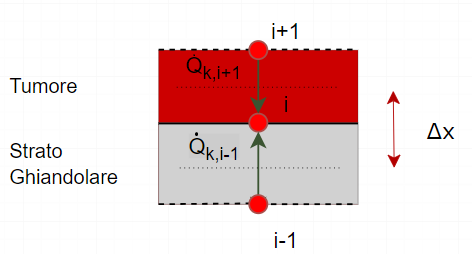
\includegraphics[width=.6\textwidth]{Immagini/Nodi/nodo15.png} 
    \label{nodo10}
\end{figure}
\noindent
Il bilancio, in questa posizione fornisce:
\begin{center}
	$ \Dot{Q} _{k, i-1} +\Dot{Q} _{k, i+1}+ \Dot{Q} _{m} +\Dot{Q} _{p}+ w_b (T) \rho _b c_b (T_b(\theta)-T_i ^?)= \frac{\Delta u}{\Delta \theta} $
\end{center}
\vspace{0.15cm}
\begin{center}
	$ \frac{k_{g} A }{\Delta x}(T_{i-1} ^? - T_i ^? ) + \frac{k_t A }{\Delta x}(T_{i+1} ^? - T_i ^? )+ \Dot{Q} _{m} + SAR_i \frac{\rho _{g} + \rho _t}{2} \Delta x + w_b (T) \rho _b c_b (T_b(\theta)-T_i ^?) = \frac{\Delta x}{ 2 \Delta \theta}(T_i ^{t+1} - T_i ^t ) (\rho _{g} c_{g} + \rho _{t} c_{t} )$
\end{center}
Definiamo il numero di Fourier in corrispondenza del tumore:
\begin{center}
	$Fo_{t}= \frac{k_{t} \Delta \theta}{\rho _{t} c_{t} \Delta x^2}$
\end{center}
Definiamo il numero di Fourier in corrispondenza dello strato ghiandolare:
\begin{center}
	$Fo_{g}= \frac{k_{g} \Delta \theta}{\rho _{g} c_{g} \Delta x^2}$
\end{center}
Un ulteriore parametro da introdurre per semplificare la scrittura equivalente un il numero di Fourier equivalente che tiene conto, contemporaneamente della sottocute e dello strato ghiandolare:
\begin{center}
	$\frac{1}{Fo_{tg}}= \frac{1}{Fo_{g}k_t}+ \frac{1}{Fo_{t}k_{g}}$
\end{center}
Da queste definizione si ottiene:
\begin{center}
	$T_i ^{t+1} $
\end{center}
\begin{center}
	$\Downarrow$
\end{center}
\begin{center}
	$T_i ^t + Fo_{tg} \Bigg[ 2\frac{T_{i+1} ^?}{k_g} + 2\frac{T_{i-1} ^?}{k_{t}}- 2T_i ^? \Big(\frac{1}{k_t} + \frac{1}{k_{g}}+ \frac{ w_b (T) \rho _b c_b \Delta x }{k_{t}k_g} \Big) +  \frac{\Delta x }{k_{t}k_g} \Big(2\Dot{Q} _{m} +  SAR_i (\rho _{t}+ \rho _g) \Delta x + 2w_b (T) \rho _b c_b T_b(\theta)\Big) \Bigg]$
\end{center}

%%%%%%%%%%%%%%%%%%%%%%%%%%%%%%%%%%%%%%%%%%%%%%%%%%%%%%%%%%%%%%%%%%
%%%%%%%%%%%%%%%%%%%%%%%%%%%%NODO 16%%%%%%%%%%%%%%%%%%%%%%%%%%%%%%%%
\subsubsection*{Nodo 16}
Il nodo 16 è posto in corrispondenza dello strato ghiandolare.\\
In questa posizione il nodo i+1 può stare in due configurazioni differenti:
\begin{enumerate}
    \item in corrispondenza dell'interfaccia tra tumore e strato ghiandolare;
    \item in corrispondenza dello strato ghiandolare.
\end{enumerate}
Di seguito vengono analizzate le due casistiche.
\begin{description}
    \item[I CASO: i+1 all'interfaccia tumore-strato ghiandolare]
    \begin{figure}[H]
    \centering
    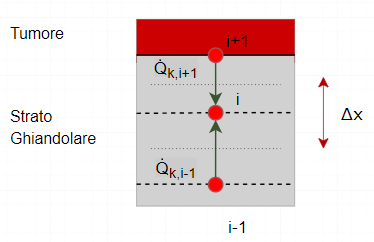
\includegraphics[width=.6\textwidth]{Immagini/Nodi/nodo16.1.png} 
    \label{nodo16.1}
\end{figure}
\noindent
\newpage
Il bilancio, in questa posizione fornisce:
\begin{center}
	$ \Dot{Q} _{k, i-1} +\Dot{Q} _{k, i+1}+ \Dot{Q} _{m} +\Dot{Q} _{p}+ w_b (T) \rho _b c_b (T_b(\theta)-T_i ^?)= \frac{\Delta U}{\Delta \theta} $
\end{center}
Con le opportune semplificazioni, si ottiene:
\begin{center}
	$T_i ^{t+1} $
\end{center}
\begin{center}
	$\Downarrow$
\end{center}
\begin{center}
	$T_i ^t + Fo_{g} \Bigg[ T_{i+1} ^? (\frac{k_g+ k_{t}}{2 \: k_g}) + T_{i-1} ^?- T_i ^? \Big(\frac{k_g+ k_{t}}{2 \: k_g} + 1 + \frac{ w_b (T) \rho _b c_b \Delta x }{k_{g}} \Big) + \frac{\Delta x }{k_{g}} \Big(\Dot{Q} _{m} +  SAR_i \rho _{g} \Delta x + w_b (T) \rho _b c_b T_b(\theta)\Big) \Bigg]$
\end{center}


\item[II CASO: i+1 nel tumore]

     \begin{figure}[H]
    \centering
    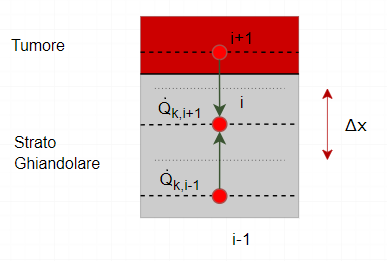
\includegraphics[width=.6\textwidth]{Immagini/Nodi/nodo16.2.png} 
    \label{nodo2}
\end{figure}
\end{description}
Il bilancio, in questa posizione fornisce:
\begin{center}
	$ \Dot{Q} _{k, i-1} +\Dot{Q} _{k, i+1}+ \Dot{Q} _{m} +\Dot{Q} _{p}+ w_b (T) \rho _b c_b (T_b(\theta)-T_i ^?)= \frac{\Delta U}{\Delta \theta} $
\end{center}
Con le opportune semplificazioni, si ottiene:
\begin{center}
	$T_i ^{t+1} $
\end{center}
\begin{center}
	$\Downarrow$
\end{center}
\begin{center}
	$T_i ^t + Fo_{g} \Bigg[ T_{i+1} ^? (\frac{k_{t}}{k_g}) + T_{i-1} ^?- T_i ^? \Big(\frac{k_{t}}{k_g} + 1 + \frac{ w_b (T) \rho _b c_b \Delta x }{k_{g}} \Big) + \frac{\Delta x }{k_{g}} \Big(\Dot{Q} _{m} +  SAR_i \rho _{g} \Delta x + w_b (T) \rho _b c_b T_b(\theta)\Big) \Bigg]$
\end{center}

%%%%%%%%%%%%%%%%%%%%%%%%%%%%%%%%%%%%%%%%%%%%%%%%%%%%%%%%%%%%%%%%%%
%%%%%%%%%%%%%%%%%%%%%%%%%%%%NODO 17%%%%%%%%%%%%%%%%%%%%%%%%%%%%%%%%
\subsubsection*{Nodo 17}
Il nodo 17 è posto in corrispondenza dello strato ghiandolare.\\
\begin{figure}[H]
    \centering
    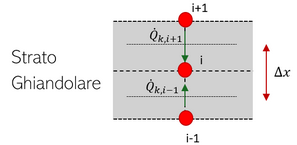
\includegraphics[width=.6\textwidth]{Immagini/Nodi/nodo17.png} 
    \label{nodo17}
\end{figure}
\noindent
Il bilancio, in questa posizione fornisce:
\begin{center}
	$ \Dot{Q} _{k, i-1} +\Dot{Q} _{k, i+1}+ \Dot{Q} _{m} +\Dot{Q} _{p}+ w_b (T) \rho _b c_b (T_b(\theta)-T_i ^?)= \frac{\Delta U}{\Delta \theta} $
\end{center}
Con le opportune semplificazioni, si ottiene:
\begin{center}
	$T_i ^{t+1} $
\end{center}
\begin{center}
	$\Downarrow$
\end{center}
\begin{center}
	$T_i ^t + Fo_{g} \Bigg[ T_{i-1} ^? + T_{i+1} ^?- T_i ^? \Big(2 + \frac{ w_b (T) \rho _b c_b \Delta x }{k_{g}} \Big) + \frac{\Delta x }{k_{g}} \Big(\Dot{Q} _{m} +  SAR_i \rho _{g} \Delta x + w_b (T) \rho _b c_b T_b(\theta)\Big) \Bigg]$
\end{center}

%%%%%%%%%%%%%%%%%%%%%%%%%%%%%%%%%%%%%%%%%%%%%%%%%%%%%%%%%%%%%%%%%%
%%%%%%%%%%%%%%%%%%%%%%%%%%%%NODO 18%%%%%%%%%%%%%%%%%%%%%%%%%%%%%%%%

\subsubsection*{Nodo 18}
Il nodo 18 è posto in corrispondenza dello strato ghiandolare.\\
In questa posizione il nodo i-1 può avere due configurazioni differenti:
\begin{enumerate}
    \item in corrispondenza dell'interfaccia tra strato ghiandolare e capillare;
    \item in corrispondenza del capillare.
\end{enumerate}
Di seguito vengono analizzate le due casistiche.
\begin{description}
    \item[I CASO: i-1 all'interfaccia strato ghiandolare - capillare]
    \begin{figure}[H]
    \centering
    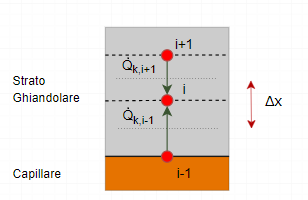
\includegraphics[width=.5\textwidth]{Immagini/Nodi/nodo18.1.png} 
    \label{nodo18.1}
\end{figure}
\noindent
\\Il bilancio, in questa posizione fornisce:
\begin{center}
	$ \Dot{Q} _{k, i-1} +\Dot{Q} _{k, i+1}+ \Dot{Q} _{m} +\Dot{Q} _{p}+ w_b (T) \rho _b c_b (T_b(\theta)-T_i ^?)= \frac{\Delta U}{\Delta \theta} $
\end{center}
Con le opportune semplificazioni, si ottiene:
\begin{center}
	$T_i ^{t+1} $
\end{center}
\begin{center}
	$\Downarrow$
\end{center}
\begin{center}
	$T_i ^t + Fo_{g} \Bigg[ T_{i-1} ^? (\frac{k_g+ k_{c}}{2 \: k_g}) + T_{i+1} ^?- T_i ^? \Big(\frac{k_g+ k_{c}}{2 \: k_g} + 1 + \frac{ w_b (T) \rho _b c_b \Delta x }{k_{g}} \Big) + \frac{\Delta x }{k_{g}} \Big(\Dot{Q} _{m} +  SAR_i \rho _{c} \Delta x + w_b (T) \rho _b c_b T_b(\theta)\Big) \Bigg]$
\end{center}


\item[II CASO: i-1 nel capillare]

     \begin{figure}[H]
    \centering
    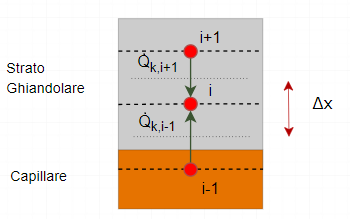
\includegraphics[width=.6\textwidth]{Immagini/Nodi/nodo18.2.png} 
    \label{nodo18.2}
\end{figure}
\end{description}
Il bilancio, in questa posizione fornisce:
\begin{center}
	$ \Dot{Q} _{k, i-1} +\Dot{Q} _{k, i+1}+ \Dot{Q} _{m} +\Dot{Q} _{p}+ w_b (T) \rho _b c_b (T_b(\theta)-T_i ^?)= \frac{\Delta U}{\Delta \theta} $
\end{center}
Con le opportune semplificazioni, si ottiene:
\begin{center}
	$T_i ^{t+1} $
\end{center}
\begin{center}
	$\Downarrow$
\end{center}
\begin{center}
	$T_i ^t + Fo_{g} \Bigg[ T_{i-1} ^? (\frac{k_{c}}{k_g}) + T_{i+1} ^?- T_i ^? \Big(\frac{k_{c}}{k_g} + 1 + \frac{ w_b (T) \rho _b c_b \Delta x }{k_{g}} \Big) + \frac{\Delta x }{k_{g}} \Big(\Dot{Q} _{m} +  SAR_i \rho _{c} \Delta x + w_b (T) \rho _b c_b T_b(\theta)\Big) \Bigg]$
\end{center}

%%%%%%%%%%%%%%%%%%%%%%%%%%%%%%%%%%%%%%%%%%%%%%%%%%%%%%%%%%%%%%%%%%
%%%%%%%%%%%%%%%%%%%%%%%%%%%%NODO 19%%%%%%%%%%%%%%%%%%%%%%%%%%%%%%%%
\subsubsection*{Nodo 19}
Il nodo 19 è posto in corrispondenza dell'interfaccia tra strato ghiandolare e capillare.
\begin{figure}[H]
    \centering
    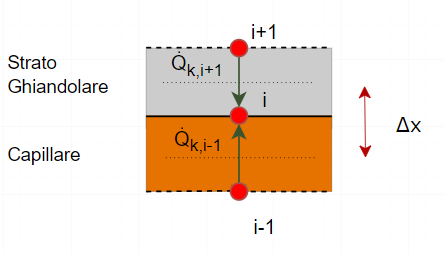
\includegraphics[width=.6\textwidth]{Immagini/Nodi/nodo19.png} 
    \label{nodo19}
\end{figure}
\noindent
Il bilancio, in questa posizione fornisce:
\begin{center}
	$ \Dot{Q} _{k, i-1} +\Dot{Q} _{k, i+1}+ \Dot{Q} _{m} +\Dot{Q} _{p}+ w_b (T) \rho _b c_b (T_b(\theta)-T_i ^?)= \frac{\Delta U}{\Delta \theta} $
\end{center}
\vspace{0.15cm}
\begin{center}
	$ \frac{k_{c} A }{\Delta x}(T_{i-1} ^? - T_i ^? ) + \frac{k_g A }{\Delta x}(T_{i+1} ^? - T_i ^? )+ \Dot{Q} _{m} + SAR_i \frac{\rho _{g} + \rho _c}{2} \Delta x + w_b (T) \rho _b c_b (T_b(\theta)-T_i ^?) = \frac{\Delta x}{ 2 \Delta \theta}(T_i ^{t+1} - T_i ^t ) (\rho _{g} c_{g} + \rho _{c} c_{c} )$
\end{center}
Definiamo il numero di Fourier in corrispondenza dello strato ghiandolare:
\begin{center}
	$Fo_{g}= \frac{k_{g} \Delta \theta}{\rho _{g} c_{g} \Delta x^2}$
\end{center}
Definiamo il numero di Fourier in corrispondenza del capillare:
\begin{center}
	$Fo_{c}= \frac{k_{c} \Delta \theta}{\rho _{c} c_{c} \Delta x^2}$
\end{center}
Un ulteriore parametro da introdurre per semplificare la scrittura equivalente un il numero di Fourier equivalente che tiene conto, contemporaneamente della sottocute e dello strato ghiandolare:
\begin{center}
	$\frac{1}{Fo_{gc}}= \frac{1}{Fo_{g}k_c}+ \frac{1}{Fo_{c}k_{g}}$
\end{center}
Da queste definizione si ottiene:
\begin{center}
	$T_i ^{t+1} $
\end{center}
\begin{center}
	$\Downarrow$
\end{center}
\begin{center}
	$T_i ^t + Fo_{gc} \Bigg[ 2\frac{T_{i+1} ^?}{k_c} + 2\frac{T_{i-1} ^?}{k_{g}}- 2T_i ^? \Big(\frac{1}{k_c} + \frac{1}{k_{g}}+ \frac{ w_b (T) \rho _b c_b \Delta x }{k_{c}k_g} \Big) +  \frac{\Delta x }{k_{c}k_g} \Big(2\Dot{Q} _{m} +  SAR_i (\rho _{c}+ \rho _g) \Delta x + 2w_b (T) \rho _b c_b T_b(\theta)\Big) \Bigg]$
\end{center}


%%%%%%%%%%%%%%%%%%%%%%%%%%%%%%%%%%%%%%%%%%%%%%%%%%%%%%%%%%%%%%%%%%
%%%%%%%%%%%%%%%%%%%%%%%%%%%%NODO 20%%%%%%%%%%%%%%%%%%%%%%%%%%%%%%%%
\subsubsection*{Nodo 20}
Il nodo 20 è posto in corrispondenza del capillare.\\
In questa posizione il nodo i+1 può stare in due configurazioni differenti:
\begin{enumerate}
    \item in corrispondenza dell'interfaccia tra strato ghiandolare e capillare;
    \item in corrispondenza dello strato ghiandolare.
\end{enumerate}
Di seguito vengono analizzate le due casistiche.
\begin{description}
    \item[I CASO: i+1 all'interfaccia strato ghiandolare - capillare]
    \begin{figure}[H]
    \centering
    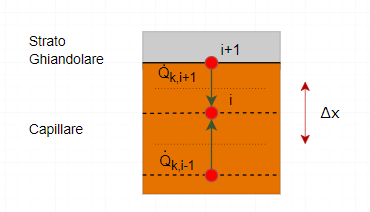
\includegraphics[width=.6\textwidth]{Immagini/Nodi/nodo20.1.png} 
    \label{nodo20.1}
\end{figure}
\noindent
\\Il bilancio, in questa posizione fornisce:
\begin{center}
	$ \Dot{Q} _{k, i-1} +\Dot{Q} _{k, i+1}+ \Dot{Q} _{m} +\Dot{Q} _{p}+ w_b (T) \rho _b c_b (T_b(\theta)-T_i ^?)= \frac{\Delta U}{\Delta \theta} $
\end{center}
Con le opportune semplificazioni, si ottiene:
\begin{center}
	$T_i ^{t+1} $
\end{center}
\begin{center}
	$\Downarrow$
\end{center}
\begin{center}
	$T_i ^t + Fo_{c} \Bigg[ T_{i+1} ^? (\frac{k_g+ k_{c}}{2 \: k_c}) + T_{i-1} ^?- T_i ^? \Big(\frac{k_g+ k_{c}}{2 \: k_c} + 1 + \frac{ w_b (T) \rho _b c_b \Delta x }{k_{c}} \Big) + \frac{\Delta x }{k_{c}} \Big(\Dot{Q} _{m} +  SAR_i \rho _{c} \Delta x + w_b (T) \rho _b c_b T_b(\theta)\Big) \Bigg]$
\end{center}


\item[II CASO: i+1 nello strato ghiandolare]

     \begin{figure}[H]
    \centering
    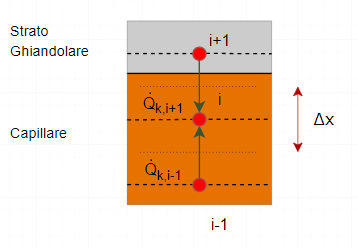
\includegraphics[width=.6\textwidth]{Immagini/Nodi/nodo20.2.png} 
    \label{nodo2}
\end{figure}
\end{description}
Il bilancio, in questa posizione fornisce:
\begin{center}
	$ \Dot{Q} _{k, i-1} +\Dot{Q} _{k, i+1}+ \Dot{Q} _{m} +\Dot{Q} _{p}+ w_b (T) \rho _b c_b (T_b(\theta)-T_i ^?)= \frac{\Delta U}{\Delta \theta} $
\end{center}
Con le opportune semplificazioni, si ottiene:
\begin{center}
	$T_i ^{t+1} $
\end{center}
\begin{center}
	$\Downarrow$
\end{center}
\begin{center}
	$T_i ^t + Fo_{c} \Bigg[ T_{i+1} ^? (\frac{k_{g}}{k_c}) + T_{i-1} ^?- T_i ^? \Big(\frac{k_{g}}{k_c} + 1 + \frac{ w_b (T) \rho _b c_b \Delta x }{k_{c}} \Big) + \frac{\Delta x }{k_{c}} \Big(\Dot{Q} _{m} +  SAR_i \rho _{c} \Delta x + w_b (T) \rho _b c_b T_b(\theta)\Big) \Bigg]$
\end{center}


%%%%%%%%%%%%%%%%%%%%%%%%%%%%%%%%%%%%%%%%%%%%%%%%%%%%%%%%%%%%%%%%%%
%%%%%%%%%%%%%%%%%%%%%%%%%%%%NODO 21%%%%%%%%%%%%%%%%%%%%%%%%%%%%%%%%
\subsubsection*{Nodo 21}
Il nodo 21 è posto in corrispondenza del capillare.\\
\begin{figure}[H]
    \centering
    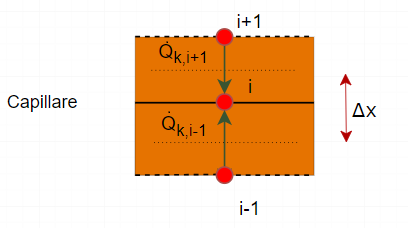
\includegraphics[width=.6\textwidth]{Immagini/Nodi/nodo21.png} 
    \label{nodo17}
\end{figure}
\noindent
Il bilancio, in questa posizione fornisce:
\begin{center}
	$ \Dot{Q} _{k, i-1} +\Dot{Q} _{k, i+1}+ \Dot{Q} _{m} +\Dot{Q} _{p}+ w_b (T) \rho _b c_b (T_b(\theta)-T_i ^?)= \frac{\Delta U}{\Delta \theta} $
\end{center}
Con le opportune semplificazioni, si ottiene:
\begin{center}
	$T_i ^{t+1} $
\end{center}
\begin{center}
	$\Downarrow$
\end{center}
\begin{center}
	$T_i ^t + Fo_{c} \Bigg[ T_{i-1} ^? + T_{i+1} ^?- T_i ^? \Big(2 + \frac{ w_b (T) \rho _b c_b \Delta x }{k_{c}} \Big) + \frac{\Delta x }{k_{c}} \Big(\Dot{Q} _{m} +  SAR_i \rho _{c} \Delta x + w_b (T) \rho _b c_b T_b(\theta)\Big) \Bigg]$
\end{center}


%%%%%%%%%%%%%%%%%%%%%%%%%%%%%%%%%%%%%%%%%%%%%%%%%%%%%%%%%%%%%%%%%%
%%%%%%%%%%%%%%%%%%%%%%%%%%%%NODO 22%%%%%%%%%%%%%%%%%%%%%%%%%%%%%%%%

\subsubsection*{Nodo 22}
Il nodo 22 è posto in corrispondenza dell'interfaccia tra il capillare e il flusso sanguigno.\\Il bilancio, in questa posizione fornisce:
\begin{center}
	$ \Dot{Q} _{k, i+1} +\Dot{Q} _{c, i}+ \Dot{Q} _{m} +\Dot{Q} _{p}+ w_b (T) \rho _b c_b (T_b(\theta)-T_i ^?)= \frac{\Delta U}{\Delta \theta} $
\end{center}

\vspace{0.1cm}
%\newline
\begin{center}
	$ \frac{k_{c} A }{\Delta x}(T_{i+1} ^? - T_i ^? ) + h_{b, \:\infty} (T_{b} (\theta) - T_i ^? )+ \Dot{Q} _{m} + SAR_i \rho _{c} \frac{\Delta x}{2}  + w_b (T) \rho _b c_b (T_b(\theta)-T_i ^?) = \rho _{c} c_{c} A \frac{\Delta x}{2 \Delta \theta}(T_i ^{t+1} - T_i ^t )$
\end{center}
Dividiamo per $k_{c}$, per A e moltiplichiamo per $\Delta x$ :
\begin{center}
	$(T_{i+1} ^? - T_i ^? ) + h_{b, \:\infty} \frac{\Delta x }{k_{c}} (T_{b}(\theta) - T_i ^? )+ \Dot{Q} _{m} \frac{\Delta x }{k_{c}}+ SAR_i \rho _{c} \frac{\Delta x^2}{2k_{c}}  + \frac{ w_b (T) \rho _b c_b \Delta x }{k_{c}}(T_b(\theta)-T_i ^?) = \rho _{c} c_{c}\frac{\Delta x^2}{2 k_{c} \Delta \theta}(T_i ^{t+1} - T_i ^t )$
\end{center}
\vspace{0.1cm}
%\newline
\noindent
Definiamo il numero di Biot locale in corrispondenza del capillare:\\
\begin{center}
	$Bi_{c}= h_{b, \:\infty} \frac{\Delta x }{k_{c}}$
\end{center}
Definiamo il numero di Fourier in corrispondenza del capillare:
\begin{center}
	$Fo_{c}= \frac{k_{c} \Delta \theta}{\rho _{c} c_{c} \Delta x^2}$
\end{center}
Sfruttando le costanti appena definite, è possibile riscrive il bilancio come segue:
\begin{center}
	$(T_{i+1} ^? - T_i ^? ) + Bi_{c} (T_{b}(\theta) - T_i ^? )+ \Dot{Q} _{m} \frac{\Delta x }{k_{c}}+ SAR_i \rho _{c} \frac{\Delta x^2}{2k_{c}}  + \frac{ w_b (T) \rho _b c_b \Delta x }{k_{c}}(T_b(\theta)-T_i ^?) = \frac{1}{2 Fo_{c}}(T_i ^{t+1} - T_i ^t )$
\end{center}
Da qui ricaviamo:
\begin{center}
	$T_i ^{t+1}$
 \begin{center}
    \begin{center}
        $\Downarrow$
    \end{center}
 \end{center}
 $T_i ^t + 2 Fo_{c} \Bigg[ T_{i+1} ^? - T_i ^? \Big(1 + Bi_{c} +  \frac{ w_b (T) \rho _b c_b \Delta x }{k_{c}} \Big) + Bi_{c} T_{b}(\theta) +  \frac{\Delta x }{k_{c}} \Big(\Dot{Q} _{m} +  SAR_i \rho _{c} \frac{\Delta x}{2} + w_b (T) \rho _b c_b T_b(\theta)\Big) \Bigg]$
\end{center}


\begin{figure}[H]
    \centering
    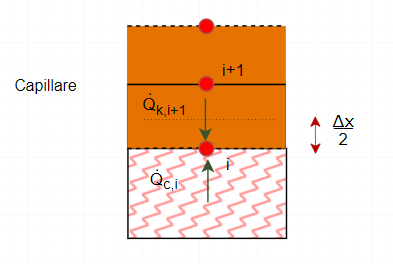
\includegraphics[width=.4\textwidth]{Immagini/Nodi/nodo22.png} 
    \label{nodo22}
\end{figure}

\newpage


\section*{Bilanci (secondo approccio delle resistenze)}

\begin{figure}[H]
	\centering
	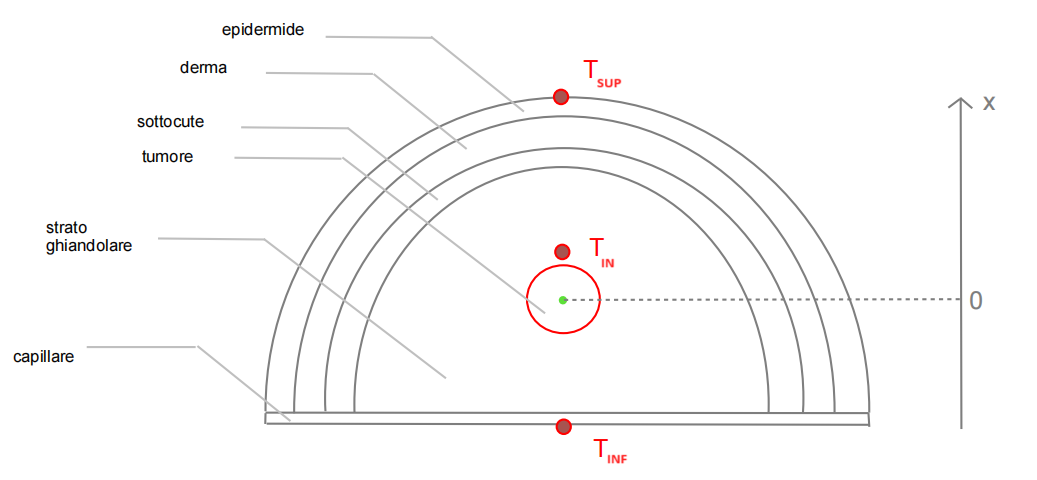
\includegraphics[width=.6\textwidth]{Immagini/sistema_3Nodi.png} 
	\label{sistema3Nodi}
\end{figure}


\subsubsection*{Bilancio nodo $T_3$ (aria-strato)}


%% Nodo T_3

\begin{center}
	$ \Dot{Q} _{k, i-1} +\Dot{Q} _{c, i}+ \Dot{Q} _{m} +\Dot{Q} _{p}+ w_b (T_i^?) \rho _b c_b (T_b(\theta)-T_i ^?)= \frac{\Delta U}{\Delta \theta} $
\end{center}

\begin{center}
	$ \frac{(T_{i-1} ^? - T_i ^? )}{R_{i-1}} + h_{c, \:\infty} (T_{\infty} (\theta) - T_i ^? )+ \Dot{Q} _{m,i} + SAR_i \: \rho _{i} \: \frac{\Delta x}{2}  + w_b (T_i^?) \rho _b \: c_b \: (T_b(\theta)-T_i ^?) = \sum_{i=1}^N \: \left( \rho _{i} \: c_{i} \: s_i \right) \: \frac{(T_i ^{t+1} - T_i ^t )}{\Delta \theta}$
\end{center}

\begin{center}
	$ \frac{(T_{i-1} ^? - T_i ^? )}{R_{i-1}} + h_{c, \:\infty} (T_{\infty} (\theta) - T_i ^? )+ \Dot{Q} _{m,i} + SAR_i \: \rho _{i} \: \frac{\Delta x}{2}  + w_b (T_i^?) \rho _b \: c_b \: (T_b(\theta)-T_i ^?) =  \: \frac{(T_i ^{t+1} - T_i ^t )}{\Sigma_3}$
\end{center}

\begin{center}
	$T_i ^{t+1}$
	\begin{center}
		\begin{center}
			$\Downarrow$
		\end{center}
	\end{center}
	$T_i ^t + \Sigma_3 \Bigg[ \frac{T_{i-1}^?}{R_{i-1}} \:-\: T_i ^? \:\Big(\frac{1}{R_{i-1}} \:+\: h_{c, \infty} \:+\:  w_b (T_i^?) \: \rho _b \: c_b  \Big) \:+\: \Dot{Q}_{m,i} \:+\: SAR_i \: \rho_i \: \frac{\Delta x}{2} \:+\: h_{c, \infty} \: T_{\infty} \:+\:  w_b (T_i^?) \rho _b c_b T_b(\theta)\Big) \Bigg]$
\end{center}

\vspace{1cm}

\subsubsection*{Bilancio nodo $T_2$ (strato-strato)}
%% Nodo T_2

\begin{center}
	$ \Dot{Q} _{k, i+1} \:+\: \Dot{Q} _{k, i-1} \:+\: \Dot{Q} _{m} +\Dot{Q} _{p}+ w_b (T_i^?) \rho _b c_b (T_b(\theta)-T_i ^?)= \frac{\Delta U}{\Delta \theta} $
\end{center}

\begin{center}
	$ \frac{(T_{i+1} ^? - T_i ^? )}{R_{i+1}} \:+\:  \frac{(T_{i-1} ^? - T_i ^? )}{R_{i-1}} \:+\: \Dot{Q} _{m,i} + SAR_i \: \rho _{i} \: \Delta x  \:+\: w_b (T_i^?) \rho _b \: c_b \: (T_b(\theta)-T_i ^?) = \sum_{i=1}^N \: \left( \rho _{i} \: c_{i} \: s_i \right) \: \frac{(T_i ^{t+1} - T_i ^t )}{\Delta \theta}$
\end{center}

\begin{center}
	$ \frac{(T_{i+1} ^? - T_i ^? )}{R_{i+1}} \:+\:  \frac{(T_{i-1} ^? - T_i ^? )}{R_{i-1}} \:+\: \Dot{Q} _{m,i} + SAR_i \: \rho _{i} \: \Delta x  \:+\: w_b (T_i^?) \rho _b \: c_b \: (T_b(\theta)-T_i ^?) =  \: \frac{(T_i ^{t+1} - T_i ^t )}{\Sigma_2}$
\end{center}

\begin{center}
	$T_i ^{t+1}$
	\begin{center}
		\begin{center}
			$\Downarrow$
		\end{center}
	\end{center}
	$T_i ^t + \Sigma_2 \Bigg[ \frac{T_{i+1}^?}{R_{i+1}} \:+\: \frac{T_{i-1}^?}{R_{i-1}} \:-\: T_i ^? \:\Big(\frac{1}{R_{i+1}} \:+\: \frac{1}{R_{i-1}} \:+\:  w_b (T_i^?) \: \rho _b \: c_b  \Big) \:+\: \Dot{Q}_{m,i} \:+\: SAR_i \: \rho_i \: \Delta x \:+\:  w_b (T_i^?) \rho _b c_b T_b(\theta)\Big) \Bigg]$
\end{center}

\vspace{0.5cm}

\subsubsection*{Bilancio nodo $T_1$ (strato-sangue)}
%% Nodo T_1

\begin{center}
	$ \Dot{Q} _{k, i+1} +\Dot{Q} _{c, i}+ \Dot{Q} _{m} +\Dot{Q} _{p}+ w_b (T_i^?) \rho _b c_b (T_b(\theta)-T_i ^?)= \frac{\Delta U}{\Delta \theta} $
\end{center}

\begin{center}
	$ \frac{(T_{i+1} ^? - T_i ^? )}{R_{i+1}} + h_{b, \:\infty} (T_{b, \infty} (\theta) - T_i ^? )+ \Dot{Q} _{m,i} + SAR_i \: \rho _{i} \: \frac{\Delta x}{2}  + w_b (T_i^?) \rho _b \: c_b \: (T_b(\theta)-T_i ^?) = \sum_{i=1}^N \: \left( \rho _{i} \: c_{i} \: s_i \right) \: \frac{(T_i ^{t+1} - T_i ^t )}{\Delta \theta}$
\end{center}

\begin{center}
	$ \frac{(T_{i+1} ^? - T_i ^? )}{R_{i+1}} + h_{b, \:\infty} (T_{b, \infty} (\theta) - T_i ^? )+ \Dot{Q} _{m,i} + SAR_i \: \rho _{i} \: \frac{\Delta x}{2}  + w_b (T_i^?) \rho _b \: c_b \: (T_b(\theta)-T_i ^?) =  \: \frac{(T_i ^{t+1} - T_i ^t )}{\Sigma_1}$
\end{center}

\begin{center}
	$T_i ^{t+1}$
	\begin{center}
		\begin{center}
			$\Downarrow$
		\end{center}
	\end{center}
	$T_i ^t + \Sigma_1 \Bigg[ \frac{T_{i+1}^?}{R_{i+1}} \:-\: T_i ^? \:\Big(\frac{1}{R_{i+1}} \:+\: h_{b, \infty} \:+\:  w_b (T_i^?) \: \rho _b \: c_b  \Big) \:+\: \Dot{Q}_{m,i} \:+\: SAR_i \: \rho_i \: \frac{\Delta x}{2} \:+\: h_{b, \infty} \: T_{b, \infty} \:+\:  w_b (T_i^?) \rho _b c_b T_b(\theta)\Big) \Bigg]$
\end{center}

\vspace{1cm}

\noindent
Il \textit{sistema di equazioni} risulta il seguente:\\

\hspace{-2.5cm}
\begin{minipage}{\textwidth}
	{\footnotesize
	\begin{align*}
		% T 1 %%%%%%%%%%%%%%%%%%%%%%%%%%%%%%%%%%%%%%%%%%%%%%%%%%%%%%%%%%%%%%%%%%%%%%%%%%%%%
		\mbox{\textcolor{blue}{$\mathbf{T_{1}}$}} \;\;
		T_{1}^{t+1} \;&=\; T_1 ^t + \Bigg[ \frac{\Sigma_1}{R_{2}}  \: T_{2}^? \:-\: T_1 ^? \:\Big(\frac{\Sigma_1}{R_{2}} \:+\:\Sigma_1 \: h_{b, \infty} \:+\:  \Sigma_1 \: w_b (T_1^?) \: \rho _b \: c_b  \Big) \:+\: \Sigma_1 \:\Dot{Q}_{m,1} \:+\: \Sigma_1 \: SAR_1 \: \rho_1 \: \frac{\Delta x}{2} \:+\: \Sigma_1 \: h_{b, \infty} \: T_{b, \infty} \:+\: \Sigma_1 \:  w_b (T_1^?) \rho _b c_b T_b(\theta)\Big) \Bigg] \\
		% T 2 %%%%%%%%%%%%%%%%%%%%%%%%%%%%%%%%%%%%%%%%%%%%%%%%%%%%%%%%%%%%%%%%%%%%%%%%%%%%%
		\mbox{\textcolor{blue}{$\mathbf{T_{2}}$}} \;\;
		T_{2}^{t+1} \;&=\; T_2 ^t + \Bigg[ \frac{\Sigma_2 }{R_{3}}T_{3}^? \:+\: \frac{\Sigma_2 }{R_{1}}T_{1}^? \:-\: T_2 ^? \:\Big(\frac{\Sigma_2}{R_{3}} \:+\: \frac{\Sigma_2 \:}{R_{1}} \:+\:  \Sigma_2 \:w_b (T_2^?) \: \rho _b \: c_b  \Big) \:+\: \Sigma_2 \:\Dot{Q}_{m,2} \:+\: \Sigma_2 \:SAR_2 \: \rho_2 \: \Delta x \:+\:  \Sigma_2 \: w_b (T_2^?) \rho _b c_b T_b(\theta)\Big) \Bigg]\\
		% T 3 %%%%%%%%%%%%%%%%%%%%%%%%%%%%%%%%%%%%%%%%%%%%%%%%%%%%%%%%%%%%%%%%%%%%%%%%%%%%%
		\mbox{\textcolor{blue}{$\mathbf{T_{3}}$}} \;\;
		T_{3}^{t+1} \;&=\; T_3 ^t + \Bigg[ \frac{\Sigma_3}{R_{2}}\: T_{2}^? \:-\: T_3 ^? \:\Big(\frac{\Sigma_3\: }{R_{2}} \:+\: \Sigma_3\: h_{c, \infty} \:+\:  \Sigma_3\: w_b (T_3^?) \: \rho _b \: c_b  \Big) \:+\: \Sigma_3\: \Dot{Q}_{m,3} \:+\: \Sigma_3\: SAR_3 \: \rho_3 \: \frac{\Delta x}{2} \:+\: \Sigma_3\: h_{c, \infty} \: T_{\infty} \:+\:  \Sigma_3\: w_b (T_3^?) \rho _b c_b T_b(\theta)\Big) \Bigg] \\
	\end{align*}
	}
\end{minipage}




\noindent
\\\\\\Tale sistema può essere riscritto in forma matriciale:\\
$$
\underline{T}^{t+1} \;=\; \underline{T}^{t} \;+\;  \underline{\underline{A}} \:  \underline{T}^{?} \;+\;  \underline{b} 
$$


\noindent
dove:
\begin{itemize}[label=·, topsep=0pt, partopsep=0pt, parsep=0pt, itemsep=0pt]
	\item \textit{$\underline{T}^{t+1}$} : vettore delle temperature all'istante t+1 ;
	\item \textit{$\underline{T}^{t}$} : vettore delle temperature all'istante t ;
	\item \textit{$\underline{\underline{A}}$} : matrice dei coefficienti;
	\item \textit{$\underline{T}^{?}$} : vettore delle temperature incognite;
	\item \textit{$\underline{b}$} : vettore dei termini noti;
\end{itemize}


\newpage


\begin{landscape} 

\thispagestyle{empty}


%\hspace{4cm}
%\scalebox{2.5}{
%	\rotatebox{270}{% Angolo di rotazione
	\scalebox{2.7}{
		\hspace{-0.7cm}
		\begin{minipage}{10cm}
			\vspace{2cm}
			\hspace{1.9cm}
			\noindent
			\tiny{\textbf{Rappresentazione matriciale del sistema\\}}
			
			\hspace{-0.5cm}
			\begin{minipage}{\columnwidth}
			$$
            \underline{T}^{t+1} \;=\; \underline{T}^{t} \;+\;  \underline{\underline{A}} \:  \underline{T}^{?} \;+\;  \underline{b} 
            $$
			\end{minipage}		
				
			\vspace{-0.5cm}
			
			\Large{ 
				\begin{gather*}
					\underbrace{
						\begin{bmatrix}
							\phantom{   }\\
							T_1^{\; t+1} \\
							T_2^{\; t+1} \\
							T_3^{\; t+1} 
						\end{bmatrix}
					}_{\underline{T}^{t+1}}
					=
					\underbrace{
						\begin{bmatrix}
							\phantom{   }\\
							T_1^{\; t} \\
							T_2^{\; t} \\
							T_3^{\; t} 
						\end{bmatrix}
					}_{\underline{T}^{t}}
					\;\;+\;\; \:
					\underbrace{
						\begin{array}{@{}c@{}}
							\begin{bmatrix}
								& \textcolor{blue}{\textbf{1}} & \textcolor{blue}{\textbf{2}} & \textcolor{blue}{\textbf{3}}  \\
								\textcolor{blue}{\textbf{1}} & -\Big(\frac{\Sigma_1}{R_{2}} + \Sigma_1 h_{b, \infty} +  \Sigma_1 w_b (T_1^?) \: \rho _b \: c_b  \Big) & \frac{\Sigma_1}{R_2} & 0  \\
								\textcolor{blue}{\textbf{2}} & \frac{\Sigma_2}{R_1} &  -  \Big(\frac{\Sigma_2}{R_{3}} + \frac{\Sigma_2}{R_{1}} +  \Sigma_2 w_b (T_2^?) \: \rho _b \: c_b  \Big) & \frac{\Sigma_2}{R_3} \\
								\textcolor{blue}{\textbf{3}} & 0 & \frac{\Sigma_3}{R_2} & -  \Big(\frac{\Sigma_3}{R_{2}} + \Sigma_3 h_{c, \infty} +  \Sigma_3 w_b (T_3^?) \: \rho _b \: c_b  \Big)  \\
							\end{bmatrix}
						\end{array}
					}_{\underline{\underline{A}}}
					\underbrace{
						\begin{bmatrix}
							\phantom{   }\\
							T_1^{\; ?} \\
							T_2^{\; ?} \\
							T_3^{\; ?} 
						\end{bmatrix}
					}_{\underline{T}^{?}}
					\;\;+\;\;
					\underbrace{
						\begin{bmatrix}
							\phantom{   }\\
							\Sigma_1 \Dot{Q}_{m,1} \:+\: \Sigma_1 SAR_1 \: \rho_1 \: \frac{\Delta x}{2} \:+\: \Sigma_1 h_{b, \infty} \: T_{b, \infty} \:+\:  \Sigma_1 w_b (T_1^?) \rho _b c_b T_b(\theta) \\
							\Sigma_2 \Dot{Q}_{m,2} \:+\: \Sigma_2 SAR_2 \: \rho_2 \: \Delta x \:+\:  \Sigma_2 w_b (T_2^?) \rho _b c_b T_b(\theta) \\
							\Sigma_3 \Dot{Q}_{m,3} \:+\: \Sigma_3 SAR_3 \: \rho_3 \: \frac{\Delta x}{2} \:+\: \Sigma_3 h_{c, \infty} \: T_{\infty} \:+\:  \Sigma_3 w_b (T_3^?) \rho _b c_b T_b(\theta) 
						\end{bmatrix}
					}_{\underline{b}}
			\end{gather*}}
		\end{minipage}}
%}}
\end{landscape}


\newpage

\noindent
Per generalizzare la scelta del metodo numerico da adottare, occorre modificare il sistema matriciale introducendo un parametro $\xi$ che consenta, in base al valore che assume, di definire uno tra tali metodi.\\

$$
\xi \;=\;
\begin{cases}
	0 \;\;\;\;\;\;\;\; \mbox{metodo esplicito}\\
	1/2 \;\;\;\;\; \mbox{metodo di Crank-Nicolson}\\
	1 \;\;\;\;\;\;\;\; \mbox{metodo implicito}
\end{cases}
$$

\vspace{0.3cm}

\noindent
Il sistema matriciale allora diventa:

$$
\underline{T}^{t+1} \;=\; \underline{T}^{t} \;+\;  \underline{\underline{A}} \;  \xi \; \underline{T}^{t+1} \;+\;  \underline{\underline{A}} \;  \left(1 \;-\; \xi \right) \;  \underline{T}^{t} \;+\;  \underline{b}
$$

\noindent
\\che può essere riscritto come:

$$
\underline{T}^{t+1} \; \underbrace{\left[\underline{\underline{I}} \;-\; \underline{\underline{A}} \;  \xi \right]}_{\underline{\underline{A}}_m} \;=\; \underbrace{ 
	\underline{T}^{t} \left[ \underline{\underline{I}} \;+\;  \underline{\underline{A}} \;  \left(1 \;-\; \xi \right) \right] \;+\;  \underline{b}}_{\underline{b}_m}
$$

$$
\underline{T}^{t+1} \; \underline{\underline{A}}_m \;=\; \underline{b}_m
$$

\noindent
É bene ricordare, infine, che in caso di scelta del \textit{metodo esplicito} ($\xi =0 $) vi è la necessità di dover assicurare il rispetto del \textit{vincolo di stabilità} secondo cui, in ogni nodo, il coefficiente del termine $T_i^t$ deve risultare positivo.\\
Per i tre nodi la condizione di stabilità risulterebbe:

\begin{adjustwidth}{0cm}{0cm}
	\begin{multicols}{3} % Divide la pagina in tre colonne
		%\centering
		
		
		\hspace{-3cm}
		\begin{minipage}{\columnwidth}	
			\vspace{1cm}
			$$T_1 \: \mbox{:}$$ 
		\end{minipage}
		
		\columnbreak % Passa alla seconda colonna
		
		
		\hspace{-5.5cm}
		\begin{minipage}{\columnwidth}	
			$$
			1 \;-\; \Sigma_1 \: \left(\frac{1}{R_2} \;+\; h_{b, \infty} \;+\; \omega_b (T_1^t) \rho_b c_b \right) \geq 0
			$$
			
			\vspace{-1cm}
			
			$$
			- \: 1 \;+\; \frac{\Delta \theta}{\sum_{i=1}^n \: \rho_i \: c_i \: s_i} \: \left(\frac{1}{R_2} \;+\; h_{b, \infty} \;+\; \omega_b (T_1^t) \rho_b c_b \right) \leq 0
			$$
			

		\end{minipage}
	
		\columnbreak
		
		\hspace{-1.5cm}
		\begin{minipage}{1.3\columnwidth}
			\vspace{0.7cm}
			$$
			\Rightarrow \;\;\;\; \Delta \theta \:\leq\: \frac{\sum_{i=1}^n \: \rho_i \: c_i \: s_i}{\frac{1}{R_2} \;+\; h_{b, \infty} \;+\; \omega_b (T_1^t) \rho_b c_b}
			$$
		\end{minipage}
		
	\end{multicols}
\end{adjustwidth}

\begin{adjustwidth}{0cm}{0cm}
	\begin{multicols}{3} % Divide la pagina in tre colonne
		%\centering
		
		
		\hspace{-3cm}
		\begin{minipage}{\columnwidth}	
			\vspace{1cm}
			$$T_2 \: \mbox{:}$$ 
		\end{minipage}
		
		\columnbreak % Passa alla seconda colonna
		
		
		\hspace{-5.5cm}
		\begin{minipage}{\columnwidth}	
			$$
			1 \;-\; \Sigma_2 \: \left(\frac{1}{R_1} \;+\; \frac{1}{R_3} \;+\; \omega_b (T_2^t) \rho_b c_b \right) \geq 0
			$$
			
			\vspace{-1cm}
			
			$$
			- \: 1 \;+\; \frac{\Delta \theta}{\sum_{i=1}^n \: \rho_i \: c_i \: s_i} \: \left(\frac{1}{R_1} \;+\; \frac{1}{R_3} \;+\; \omega_b (T_2^t) \rho_b c_b \right) \leq 0
			$$
			
			
		\end{minipage}
		
		\columnbreak
		
		\hspace{-1.5cm}
		\begin{minipage}{1.3\columnwidth}
			\vspace{0.7cm}
			$$
			\Rightarrow \;\;\;\; \Delta \theta \:\leq\: \frac{\sum_{i=1}^n \: \rho_i \: c_i \: s_i}{\frac{1}{R_1} \;+\; \frac{1}{R_3} \;+\; \omega_b (T_2^t) \rho_b c_b}
			$$
		\end{minipage}
		
	\end{multicols}
\end{adjustwidth}

\begin{adjustwidth}{0cm}{0cm}
	\begin{multicols}{3} % Divide la pagina in tre colonne
		%\centering
		
		
		\hspace{-3cm}
		\begin{minipage}{\columnwidth}	
			\vspace{1cm}
			$$T_3 \: \mbox{:}$$ 
		\end{minipage}
		
		\columnbreak % Passa alla seconda colonna
		
		
		\hspace{-5.5cm}
		\begin{minipage}{\columnwidth}	
			$$
			1 \;-\; \Sigma_3 \: \left(\frac{1}{R_2} \;+\; h_{c, \infty} \;+\; \omega_b (T_3^t) \rho_b c_b \right) \geq 0
			$$
			
			\vspace{-1cm}
			
			$$
			- \: 1 \;+\; \frac{\Delta \theta}{\sum_{i=1}^n \: \rho_i \: c_i \: s_i} \: \left(\frac{1}{R_2} \;+\; h_{c, \infty} \;+\; \omega_b (T_3^t) \rho_b c_b \right) \leq 0
			$$
			
			
		\end{minipage}
		
		\columnbreak
		
		\hspace{-1.5cm}
		\begin{minipage}{1.3\columnwidth}
			\vspace{0.7cm}
			$$
			\Rightarrow \;\;\;\; \Delta \theta \:\leq\: \frac{\sum_{i=1}^n \: \rho_i \: c_i \: s_i}{\frac{1}{R_2} \;+\; h_{c, \infty} \;+\; \omega_b (T_3^t) \rho_b c_b}
			$$
		\end{minipage}
		
	\end{multicols}
\end{adjustwidth}

\newpage

\begin{landscape} 
	
	\thispagestyle{empty}
	
	\begin{center}
	%\hspace{4cm}
	%\scalebox{2.5}{
		%	\rotatebox{270}{% Angolo di rotazione
			\scalebox{2}{
				\hspace{-0.7cm}
				\begin{minipage}{10cm}
					\vspace{2cm}
					\hspace{1.9cm}
					\noindent
					\tiny{\textbf{Rappresentazione matriciale del sistema\\}}
					
					\hspace{-0.5cm}
					\begin{minipage}{\columnwidth}
						$$
                        \underline{T}^{t+1} \; \underbrace{\left[\underline{\underline{I}} \;-\; \underline{\underline{A}} \;  \xi \right]}_{\underline{\underline{A}}_m} \;=\; \underbrace{ 
	                    \underline{T}^{t} \left[ \underline{\underline{I}} \;+\;  \underline{\underline{A}} \;  \left(1 \;-\; \xi \right) \right] \;+\;  \underline{b}}_{\underline{b}_m}
                        $$
					\end{minipage}		
					
					\vspace{-0.5cm}
					
				
					\Large{ 
						\begin{gather*}
							\underline{\underline{A}}_m
							\;=\;
							\underbrace{
								\begin{array}{@{}c@{}}
									\begin{bmatrix}
										& \textcolor{blue}{\textbf{1}} & \textcolor{blue}{\textbf{2}} & \textcolor{blue}{\textbf{3}}  \\
										\textcolor{blue}{\textbf{1}} & 1 & 0 & 0 \\
										\textcolor{blue}{\textbf{2}} & 0 & 1 & 0 \\
										\textcolor{blue}{\textbf{3}} & 0 & 0 & 1  \\
									\end{bmatrix}
								\end{array}
							}_{\underline{\underline{I}}}
							\;\;-\;\;
							\underbrace{
								\resizebox{2\textwidth}{!}{%
									$
									\begin{array}{@{}c@{}}
										\begin{bmatrix}
											& \textcolor{blue}{\textbf{1}} & \textcolor{blue}{\textbf{2}} & \textcolor{blue}{\textbf{3}}  \\
											\textcolor{blue}{\textbf{1}} & -\Big(\frac{\Sigma_1}{R_{2}} + \Sigma_1 h_{b, \infty} +  \Sigma_1 w_b (T_1^?) \: \rho _b \: c_b  \Big) & \frac{\Sigma_1}{R_2} & 0  \\
											\textcolor{blue}{\textbf{2}} & \frac{\Sigma_2}{R_1} &  -  \Big(\frac{\Sigma_2}{R_{3}} + \frac{\Sigma_2}{R_{1}} + \Sigma_2 w_b (T_2^?) \: \rho _b \: c_b  \Big) & \frac{\Sigma_2}{R_3} \\
											\textcolor{blue}{\textbf{3}} & 0 & \frac{\Sigma_3}{R_2} & -  \Big(\frac{\Sigma_3}{R_{2}} + \Sigma_3 h_{c, \infty} + \Sigma_3 w_b (T_3^?) \: \rho _b \: c_b  \Big)  \\
										\end{bmatrix}
									\end{array}
									$}
							}_{\underline{\underline{A}}}
							\; \xi
					\end{gather*}}
					
					\hspace{-1.8cm}
					\begin{minipage}{1.4\columnwidth}
					\Large{ 
						\begin{gather*}
							\underline{b}_m
							\;=\;
							\underbrace{
									\begin{bmatrix}
										\phantom{   }\\
										T_1^{\; t} \\
										T_2^{\; t} \\
										T_3^{\; t} 
									\end{bmatrix}
							}_{\underline{T}^{t}}
							\underbrace{
									\begin{array}{@{}c@{}}
										\begin{bmatrix}
											& \textcolor{blue}{\textbf{1}} & \textcolor{blue}{\textbf{2}} & \textcolor{blue}{\textbf{3}}  \\
											\textcolor{blue}{\textbf{1}} & 1 & 0 & 0  \\
											\textcolor{blue}{\textbf{2}} & 0 & 1 & 0 \\
											\textcolor{blue}{\textbf{3}} & 0 & 0 & 1  \\
										\end{bmatrix}
									\end{array}
							}_{\underline{\underline{I}}}
							\;+\;	
							\underbrace{								
									\begin{bmatrix}
										\phantom{   }\\
										T_1^{\; t} \\
										T_2^{\; t} \\
										T_3^{\; t} 
									\end{bmatrix}									
							}_{\underline{T}^{t}}
							\underbrace{
									\begin{array}{@{}c@{}}
										\begin{bmatrix}
											& \textcolor{blue}{\textbf{1}} & \textcolor{blue}{\textbf{2}} & \textcolor{blue}{\textbf{3}}  \\
											\textcolor{blue}{\textbf{1}} & -\Big(\frac{\Sigma_1}{R_{2}} + \Sigma_1 h_{b, \infty} +  \Sigma_1 w_b (T_1^?) \: \rho _b \: c_b  \Big) & \frac{\Sigma_1}{R_2} & 0  \\
											\textcolor{blue}{\textbf{2}} & \frac{\Sigma_2}{R_1} &  -  \Big(\frac{\Sigma_2}{R_{3}} + \frac{\Sigma_2}{R_{1}} + \Sigma_2 w_b (T_2^?) \: \rho _b \: c_b  \Big) & \frac{\Sigma_2}{R_3} \\
											\textcolor{blue}{\textbf{3}} & 0 & \frac{\Sigma_3}{R_2} & -  \Big(\frac{\Sigma_3}{R_{2}} + \Sigma_3 h_{c, \infty} + \Sigma_3 w_b (T_3^?) \: \rho _b \: c_b  \Big)  \\
										\end{bmatrix}
									\end{array}									
							}_{\underline{\underline{A}}}
								\; \left( 1 \;-\; \xi \right)
							\;+\;	
							\underbrace{								
									\begin{bmatrix}
										\phantom{   }\\
										\Sigma_1 \Dot{Q}_{m,1} \:+\: \Sigma_1 SAR_1 \: \rho_1 \: \frac{\Delta x}{2} \:+\: \Sigma_1 h_{b, \infty} \: T_{b, \infty} \:+\: \Sigma_1  w_b (T_1^?) \rho _b c_b T_b(\theta) \\
										\Sigma_2 \Dot{Q}_{m,2} \:+\: \Sigma_2 SAR_2 \: \rho_2 \: \Delta x \:+\:  \Sigma_2 w_b (T_2^?) \rho _b c_b T_b(\theta) \\
										\Sigma_3 \Dot{Q}_{m,3} \:+\: \Sigma_3 SAR_3 \: \rho_3 \: \frac{\Delta x}{2} \:+\: \Sigma_3 h_{c, \infty} \: T_{\infty} \:+\:  \Sigma_3 w_b (T_3^?) \rho _b c_b T_b(\theta) 
									\end{bmatrix}									
							}_{\underline{b}}
					\end{gather*}}
					\end{minipage}
				
			\end{minipage}}
			%}}
		\end{center}
\end{landscape}


\newpage


\newgeometry{a4paper, top=2.5cm, bottom=2.5cm, left=0.5cm, right=0.5cm}


\section*{\hspace{2cm} Bilanci (terzo approccio)}

\begin{figure}[H]
	\centering
	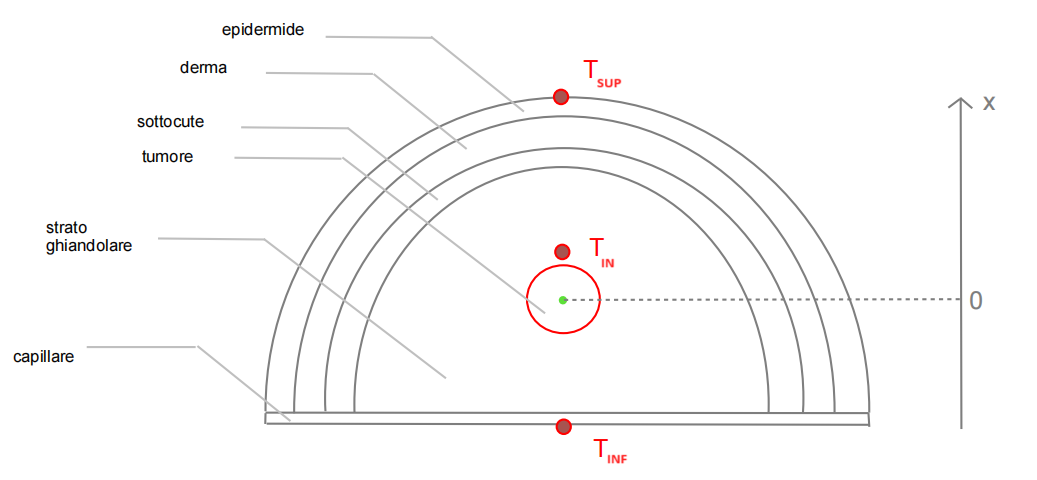
\includegraphics[width=.8\textwidth]{Immagini/sistema_3Nodi.png} 
	\label{sistema3Nodi}
\end{figure}

%% Nodo SUP
\subsubsection*{\hspace{1cm} Bilancio nodo $T_{SUP}$ (aria-strato)}

\vspace{0.3cm}

\begin{center}
	$ \Dot{Q} _{k, i-1} +\Dot{Q} _{c, i}+ \Dot{Q} _{m} +\Dot{Q} _{probe}+ \Dot{Q} _{perf}= \frac{\Delta U}{\Delta \theta} $
\end{center}

\hspace{-0.5cm}
\begin{minipage}\columnwidth
\begin{center}
	$ \frac{k_{ep}A}{\Delta x}(T_{i-1} ^? - T_i ^? ) + h_{c, \infty}A (T_{\infty} (\theta) - T_i ^? ) + \Dot{u} _{m,ep}\frac{\Delta x}{2}A + SAR_{ep} \: \rho _{ep} \: \frac{\Delta x}{2}A  + w_b (T_i^?) \rho _b \: c_b \: \frac{\Delta x}{2}A(T_b(\theta)-T_i ^?) =  \rho _{ep} \: c_{ep} \: \frac{\Delta x}{2}A \: \frac{(T_i ^{t+1} - T_i ^t )}{\Delta \theta}$
\end{center}
\end{minipage}

\hspace{-0.5cm}
\begin{minipage}\columnwidth
\begin{center}
	$ T_{i-1} ^? - T_i ^? + \frac{h_{c, \infty} \Delta x}{k_{ep}} (T_{\infty} (\theta) - T_i ^? ) + \Dot{u} _{m,ep}\:\frac{{\Delta x}^2}{2 k_{ep}} + SAR_{ep} \: \rho _{ep} \: \frac{{\Delta x}^2}{2 k_{ep}}  + w_b (T_i^?) \rho _b \: c_b \: \frac{{\Delta x}^2}{2 k_{ep}}(T_b(\theta)-T_i ^?) =  \rho _{ep} \: c_{ep} \: \frac{{\Delta x}^2}{2 k_{ep}} \: \frac{(T_i ^{t+1} - T_i ^t )}{\Delta \theta}$
\end{center}
\end{minipage}

\vspace{0.5cm}
\noindent
\hspace{2cm} Sapendo che:
\vspace{-0.3cm}

\begin{center}
    $Bi_{ep} \;=\; \frac{h_{c,\infty} \Delta x}{k_{ep}}$
\end{center}

\begin{center}
    $Fo_{ep} \;=\; \frac{k_{ep} \Delta \theta}{\rho_{ep} c_{ep} {\Delta x}^2}$
\end{center}

\vspace{0.3cm}
\noindent
\hspace{2cm} allora:
\vspace{-0.3cm}


\begin{center}
	$T_i ^{t+1}$
	\begin{center}
		\begin{center}
			$\Downarrow$
		\end{center}
	\end{center}
	$T_i ^t + 2 \: Fo_{ep} \Bigg[ T_{i-1}^? \:-\: T_i^? \:\Big(Bi_{ep} \:+\: 1 \:+\:  \frac{{\Delta x}^2 w_b (T_i^?) \: \rho _b \: c_b}{2 \: k_{ep}} \Big) \:+\: Bi_{ep} T_{\infty} \:+\: \frac{{\Delta x}^2}{2 k_{ep}} \Big(\Dot{u}_{m,ep} \;+\; SAR_{ep} \rho_{ep} \:+\:  w_b (T_i^?) \rho _b c_b T_b(\theta)\Big) \Bigg]$
\end{center}

















\newpage
















%% Nodo CENTER
\subsubsection*{\hspace{1cm} Bilancio nodo $T_{IN}$ (strato-strato)}

\vspace{0.3cm}

\begin{center}
	$ \Dot{Q} _{k, i-1} +\Dot{Q} _{k, i+1}+ \Dot{Q}_{m} +\Dot{Q} _{probe}+ \Dot{Q} _{perf}= \frac{\Delta U}{\Delta \theta} $
\end{center}

\hspace{-0.5cm}
\begin{minipage}\columnwidth
\begin{center}
	$ \frac{k_{i-1}A}{\Delta x}(T_{i-1} ^? - T_i ^? ) + \frac{k_{i+1}A}{\Delta x}(T_{i+1} ^? - T_i ^? ) + \Dot{u} _{m,i}\Delta x \: A + SAR_{i} \: \rho _{i} \: \Delta x \: A  + w_b (T_i^?) \rho _b \: c_b \: \Delta x \: A \: (T_b(\theta)-T_i ^?) = \sum_{k=1}^{n} \rho _{k} \: c_{k} \: s_{k} \: A \: \frac{(T_i ^{t+1} - T_i ^t )}{\Delta \theta}$
\end{center}
\end{minipage}



\vspace{0.5cm}
\noindent
\hspace{2cm} Sapendo che:
\vspace{-0.3cm}

\begin{center}
    $\frac{1}{\Sigma} \;=\; \frac{\sum_{k=1}^{n} \rho _{k} \: c_{k} \: s_{k}}{\Delta \theta}$
\end{center}



\vspace{0.3cm}
\noindent
\hspace{2cm} allora:
\vspace{-0.3cm}


\begin{center}
	$T_i ^{t+1}$
	\begin{center}
		\begin{center}
			$\Downarrow$
		\end{center}
	\end{center}
	$T_i ^t + \Sigma \Bigg[ \frac{k_{i-1}}{\Delta x} \: T_{i-1}^? \:+\: \frac{k_{i+1}}{\Delta x}\: T_{i+1}^? \;-\; T_i^?\:\Big(\frac{k_{i-1}}{\Delta x}  \:+\: \frac{k_{i+1}}{\Delta x} \:+\:  \Delta x \: w_b (T_i^?) \: \rho _b \: c_b \Big) \:+\: \Delta x \: \Big(\Dot{u}_{m,i} \;+\; SAR_{i} \rho_{i} \:+\:  w_b (T_i^?) \rho _b c_b T_b(\theta)\Big) \Bigg]$
\end{center}














\vspace{3cm}
























%% Nodo INF
\subsubsection*{\hspace{1cm} Bilancio nodo $T_{INF}$ (strato-capillare)}

\vspace{0.3cm}

\begin{center}
	$ \Dot{Q} _{k, i+1} +\Dot{Q} _{c, i}+ \Dot{Q} _{m} +\Dot{Q} _{probe}+ \Dot{Q} _{perf}= \frac{\Delta U}{\Delta \theta} $
\end{center}

\hspace{-0.5cm}
\begin{minipage}\columnwidth
\begin{center}
	$ \frac{k_{i+1}A}{\Delta x}(T_{i+1} ^? - T_i ^? ) + h_{b, \infty}A (T_{b} (\theta) - T_i ^? ) + \Dot{u} _{m,c}\frac{\Delta x}{2}A + SAR_{c} \: \rho _{c} \: \frac{\Delta x}{2}A  + w_b (T_i^?) \rho _b \: c_b \: \frac{\Delta x}{2}A(T_b(\theta)-T_i ^?) =  \sum_{k=1}^{n} \rho _{k} \: c_{k} \: s_{k} \: A \: \frac{(T_i ^{t+1} - T_i ^t )}{\Delta \theta}$
\end{center}
\end{minipage}




\vspace{0.5cm}
\noindent
\hspace{2cm} Sapendo che:
\vspace{-0.3cm}

\begin{center}
    $\frac{1}{\Sigma} \;=\; \frac{\sum_{k=1}^{n} \rho _{k} \: c_{k} \: s_{k}}{\Delta \theta}$
\end{center}



\vspace{0.3cm}
\noindent
\hspace{2cm} allora:
\vspace{-0.3cm}


\begin{center}
	$T_i ^{t+1}$
	\begin{center}
		\begin{center}
			$\Downarrow$
		\end{center}
	\end{center}
	$T_i ^t + \Sigma \Bigg[ \frac{k_{i+1}}{\Delta x}\: T_{i+1}^? \;-\; T_i^?\:\Big( \frac{k_{i+1}}{\Delta x} \:+\: h_{b,\infty} \;+\;  \frac{\Delta x}{2} \:  w_b (T_i^?) \: \rho _b \: c_b \Big) \:+\: h_{b, \infty} T_{\infty,b} \;+\; \frac{\Delta x}{2} \: \Big(\Dot{u}_{m,c} \;+\; SAR_{c} \rho_{c} \:+\:  w_b (T_i^?) \rho _b c_b T_b(\theta)\Big) \Bigg]$
\end{center}


\newpage

\begin{comment}
\noindent
\hspace{1cm} Affinché ci sia almeno un nodo in ogni strato, il numero minimo di nodi da dover considerare è di \textit{12 nodi}.

\begin{figure}[H]
	\centering
	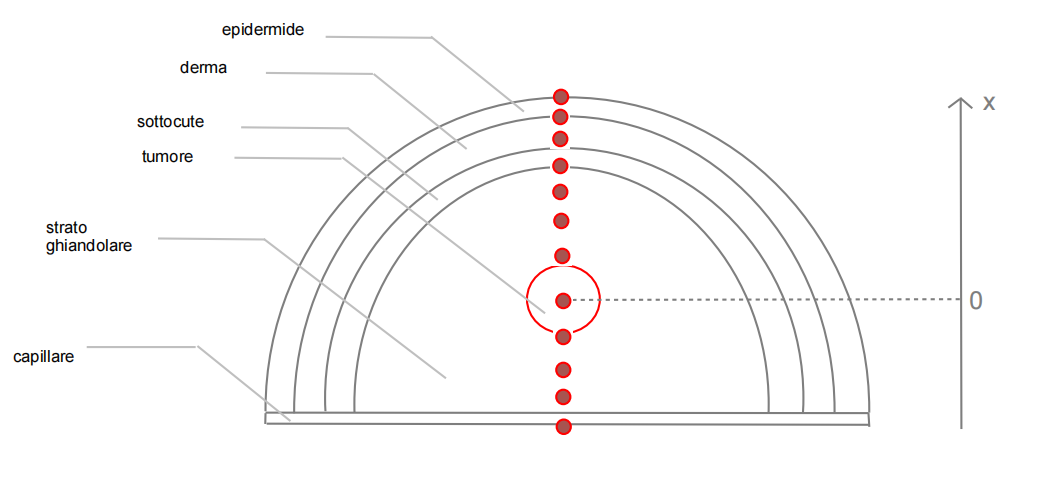
\includegraphics[width=.8\textwidth]{Immagini/sistema_12Nodi.png} 
	\label{sistema3Nodi}
\end{figure}
\end{comment}

\noindent
\hspace{1cm} Il \textit{sistema di equazioni} risulta il seguente:\\

\hspace{-1cm}
\begin{minipage}{\textwidth}
	{\footnotesize
	\begin{align*}
		% T 1 %%%%%%%%%%%%%%%%%%%%%%%%%%%%%%%%%%%%%%%%%%%%%%%%%%%%%%%%%%%%%%%%%%%%%%%%%%%%%
		\mbox{\textcolor{blue}{$\mathbf{T_{1}}$}} \;\;
		T_{1}^{t+1} \;&=\; T_1 ^t + \Sigma \Bigg[ \frac{k_{2}}{\Delta x}\: T_{2}^? \;-\; T_1^?\:\Big( \frac{k_{2}}{\Delta x} \:+\: h_{b,\infty} \;+\;  \frac{\Delta x}{2} \:  w_b (T_1^?) \: \rho _b \: c_b \Big) \:+\: h_{b, \infty} T_{\infty,b} \;+\; \frac{\Delta x}{2} \: \Big(\Dot{u}_{m,c} \;+\; SAR_{c} \rho_{c} \:+\:  w_b (T_1^?) \rho _b c_b T_b(\theta)\Big) \Bigg]\\
		% T 2 %%%%%%%%%%%%%%%%%%%%%%%%%%%%%%%%%%%%%%%%%%%%%%%%%%%%%%%%%%%%%%%%%%%%%%%%%%%%%
		\mbox{\textcolor{blue}{$\mathbf{T_{2}}$}} \;\;
		T_{2}^{t+1} \;&=\; T_2 ^t + \Sigma \Bigg[ \frac{k_{1}}{\Delta x} \: T_{1}^? \:+\: \frac{k_{3}}{\Delta x}\: T_{3}^? \;-\; T_2^?\:\Big(\frac{k_{1}}{\Delta x}  \:+\: \frac{k_{3}}{\Delta x} \:+\:  \Delta x \: w_b (T_2^?) \: \rho _b \: c_b \Big) \:+\: \Delta x \: \Big(\Dot{u}_{m,2} \;+\; SAR_{2} \rho_{2} \:+\:  w_b (T_2^?) \rho _b c_b T_b(\theta)\Big) \Bigg]\\
		% T 3 %%%%%%%%%%%%%%%%%%%%%%%%%%%%%%%%%%%%%%%%%%%%%%%%%%%%%%%%%%%%%%%%%%%%%%%%%%%%%
		\mbox{\textcolor{blue}{$\mathbf{T_{3}}$}} \;\;
		T_{3}^{t+1} \;&=\; T_3 ^t + 2 \: Fo_{ep} \Bigg[ T_{2}^? \:-\: T_3^? \:\Big(Bi_{ep} \:+\: 1 \:+\:  \frac{{\Delta x}^2 w_b (T_3^?) \: \rho _b \: c_b}{2 \: k_{ep}} \Big) \:+\: Bi_{ep} T_{\infty} \:+\: \frac{{\Delta x}^2}{2 k_{ep}} \Big(\Dot{u}_{m,ep} \;+\; SAR_{ep} \rho_{ep} \:+\:  w_b (T_3^?) \rho _b c_b T_b(\theta)\Big) \Bigg] \\
	\end{align*}
	}
\end{minipage}


\vspace{1.5cm}


\noindent
\hspace{2cm}  Tale sistema può essere riscritto in forma matriciale:\\
$$
\underline{T}^{t+1} \;=\; \underline{T}^{t} \;+\;  \underline{\underline{A}} \:  \underline{T}^{?} \;+\;  \underline{b} 
$$


\noindent
\hspace{1cm}  dove:
\begin{itemize}[label=·, topsep=0pt, partopsep=0pt, parsep=0pt, itemsep=0pt]
	\item \textit{$\underline{T}^{t+1}$} : vettore delle temperature all'istante t+1 ;
	\item \textit{$\underline{T}^{t}$} : vettore delle temperature all'istante t ;
	\item \textit{$\underline{\underline{A}}$} : matrice dei coefficienti;
	\item \textit{$\underline{T}^{?}$} : vettore delle temperature incognite;
	\item \textit{$\underline{b}$} : vettore dei termini noti;
\end{itemize}

\restoregeometry

\newpage


\begin{landscape} 

\thispagestyle{empty}


%\hspace{4cm}
%\scalebox{2.5}{
%	\rotatebox{270}{% Angolo di rotazione
	\scalebox{2.7}{
		\hspace{-0.9cm}
		\begin{minipage}{10cm}
			\vspace{2cm}
			\hspace{1.9cm}
			\noindent
			\tiny{\textbf{Rappresentazione matriciale del sistema\\}}
			
			\hspace{-0.5cm}
			\begin{minipage}{\columnwidth}
			$$
            \underline{T}^{t+1} \;=\; \underline{T}^{t} \;+\;  \underline{\underline{A}} \:  \underline{T}^{?} \;+\;  \underline{b} 
            $$
			\end{minipage}		
				
			\vspace{-0.5cm}
			
			\Large{ 
				\begin{gather*}
					\underbrace{
						\begin{bmatrix}
							\phantom{   }\\
							T_1^{\; t+1} \\
							T_2^{\; t+1} \\
							T_3^{\; t+1} 
						\end{bmatrix}
					}_{\underline{T}^{t+1}}
					=
					\underbrace{
						\begin{bmatrix}
							\phantom{   }\\
							T_1^{\; t} \\
							T_2^{\; t} \\
							T_3^{\; t} 
						\end{bmatrix}
					}_{\underline{T}^{t}}
					\;\;+\;\; \:
					\underbrace{
						\begin{array}{@{}c@{}}
							\begin{bmatrix}
								& \textcolor{blue}{\textbf{1}} & \textcolor{blue}{\textbf{2}} & \textcolor{blue}{\textbf{3}}  \\
								\textcolor{blue}{\textbf{1}} & -\Sigma_1 \Big( \frac{k_{2}}{\Delta x} \:+\: h_{b,\infty} \;+\;  \frac{\Delta x}{2} \:  w_b (T_1^?) \: \rho _b \: c_b \Big) & \Sigma_1 \frac{k_{2}}{\Delta x} & 0  \\
								\textcolor{blue}{\textbf{2}} & \Sigma_2 \frac{k_{1}}{\Delta x} &  -\Sigma_2 \Big(\frac{k_{1}}{\Delta x}  \:+\: \frac{k_{3}}{\Delta x} \:+\:  \Delta x \: w_b (T_2^?) \: \rho _b \: c_b \Big) & \Sigma_2 \frac{k_{3}}{\Delta x}\\
								\textcolor{blue}{\textbf{3}} & 0 & 2 \: Fo_{ep} & - 2 \: Fo_{ep} \Big(Bi_{ep} \:+\: 1 \:+\:  \frac{{\Delta x}^2 w_b (T_3^?) \: \rho _b \: c_b}{2 \: k_{ep}} \Big) \\
							\end{bmatrix}
						\end{array}
					}_{\underline{\underline{A}}}
					\underbrace{
						\begin{bmatrix}
							\phantom{   }\\
							T_1^{\; ?} \\
							T_2^{\; ?} \\
							T_3^{\; ?} 
						\end{bmatrix}
					}_{\underline{T}^{?}}
					\;\;+\;\;
					\underbrace{
						\begin{bmatrix}
							\phantom{   }\\
							\Sigma_1 \left[h_{b, \infty} T_{\infty,b} \;+\; \frac{\Delta x}{2} \: \Big(\Dot{u}_{m,c} \;+\; SAR_{c} \rho_{c} \:+\:  w_b (T_1^?) \rho _b c_b T_b(\theta)\Big)\right] \\
							\Sigma_2 \Delta x \: \Big(\Dot{u}_{m,2} \;+\; SAR_{2} \rho_{2} \:+\:  w_b (T_2^?) \rho _b c_b T_b(\theta)\Big) \\
							2 \: Fo_{ep} \left[Bi_{ep} T_{\infty} \:+\: \frac{{\Delta x}^2}{2 k_{ep}} \Big(\Dot{u}_{m,ep} \;+\; SAR_{ep} \rho_{ep} \:+\:  w_b (T_3^?) \rho _b c_b T_b(\theta)\Big)\right]
						\end{bmatrix}
					}_{\underline{b}}
			\end{gather*}}
		\end{minipage}}
%}}
\end{landscape}


\newpage



\noindent
Per generalizzare la scelta del metodo numerico da adottare, occorre modificare il sistema matriciale introducendo un parametro $\xi$ che consenta, in base al valore che assume, di definire uno tra tali metodi.\\

$$
\xi \;=\;
\begin{cases}
	0 \;\;\;\;\;\;\;\; \mbox{metodo esplicito}\\
	1/2 \;\;\;\;\; \mbox{metodo di Crank-Nicolson}\\
	1 \;\;\;\;\;\;\;\; \mbox{metodo implicito}
\end{cases}
$$

\vspace{0.3cm}

\noindent
Il sistema matriciale allora diventa:

$$
\underline{T}^{t+1} \;=\; \underline{T}^{t} \;+\;  \underline{\underline{A}} \;  \xi \; \underline{T}^{t+1} \;+\;  \underline{\underline{A}} \;  \left(1 \;-\; \xi \right) \;  \underline{T}^{t} \;+\;  \underline{b}
$$

\noindent
\\che può essere riscritto come:

$$
\underline{T}^{t+1} \; \underbrace{\left[\underline{\underline{I}} \;-\; \underline{\underline{A}} \;  \xi \right]}_{\underline{\underline{A}}_m} \;=\; \underbrace{ 
	\underline{T}^{t} \left[ \underline{\underline{I}} \;+\;  \underline{\underline{A}} \;  \left(1 \;-\; \xi \right) \right] \;+\;  \underline{b}}_{\underline{b}_m}
$$

$$
\underline{T}^{t+1} \; \underline{\underline{A}}_m \;=\; \underline{b}_m
$$

\noindent
É bene ricordare, infine, che in caso di scelta del \textit{metodo esplicito} ($\xi =0 $) vi è la necessità di dover assicurare il rispetto del \textit{vincolo di stabilità} secondo cui, in ogni nodo, il coefficiente del termine $T_i^t$ deve risultare positivo.\\
Per i tre nodi la condizione di stabilità risulterebbe:

\begin{adjustwidth}{0cm}{0cm}
	\begin{multicols}{3} % Divide la pagina in tre colonne
		%\centering
		
		
		\hspace{-3cm}
		\begin{minipage}{\columnwidth}	
			\vspace{1cm}
			$$T_1 \: \mbox{:}$$ 
		\end{minipage}
		
		\columnbreak % Passa alla seconda colonna
		
		
		\hspace{-5.5cm}
		\begin{minipage}{\columnwidth}	
			$$
			1 \;-\; \Sigma_1 \Big( \frac{k_{2}}{\Delta x} \:+\: h_{b,\infty} \;+\;  \frac{\Delta x}{2} \:  w_b (T_1^?) \: \rho _b \: c_b \Big) \geq 0
			$$
			
			\vspace{-1cm}
			
			$$
			- \: 1 \;+\; \Sigma_1 \Big( \frac{k_{2}}{\Delta x} \:+\: h_{b,\infty} \;+\;  \frac{\Delta x}{2} \:  w_b (T_1^?) \: \rho _b \: c_b \Big) \leq 0
			$$
			

		\end{minipage}
	
		\columnbreak
		
		\hspace{-1.5cm}
		\begin{minipage}{1.3\columnwidth}
			\vspace{0.7cm}
			$$
			\Rightarrow \;\;\;\; \Delta \theta \:\leq\: \frac{\sum_{k=1}^n \: \rho_k \: c_k \: s_k}{\frac{k_{2}}{\Delta x} \:+\: h_{b,\infty} \;+\;  \frac{\Delta x}{2} \:  w_b (T_1^?) \: \rho _b \: c_b}
			$$
		\end{minipage}
		
	\end{multicols}
\end{adjustwidth}

\begin{adjustwidth}{0cm}{0cm}
	\begin{multicols}{3} % Divide la pagina in tre colonne
		%\centering
		
		
		\hspace{-3cm}
		\begin{minipage}{\columnwidth}	
			\vspace{1cm}
			$$T_2 \: \mbox{:}$$ 
		\end{minipage}
		
		\columnbreak % Passa alla seconda colonna
		
		
		\hspace{-5.5cm}
		\begin{minipage}{\columnwidth}	
			$$
			1 \;-\Sigma_2 \Big(\frac{k_{1}}{\Delta x}  \:+\: \frac{k_{3}}{\Delta x} \:+\:  \Delta x \: w_b (T_2^?) \: \rho _b \: c_b \Big) \geq 0
			$$
			
			\vspace{-1cm}
			
			$$
			- \: 1 \;+\; \Sigma_2 \Big(\frac{k_{1}}{\Delta x}  \:+\: \frac{k_{3}}{\Delta x} \:+\:  \Delta x \: w_b (T_2^?) \: \rho _b \: c_b \Big) \leq 0
			$$
			
			
		\end{minipage}
		
		\columnbreak
		
		\hspace{-1.5cm}
		\begin{minipage}{1.3\columnwidth}
			\vspace{0.7cm}
			$$
			\Rightarrow \;\;\;\; \Delta \theta \:\leq\: \frac{\sum_{i=1}^n \: \rho_i \: c_i \: s_i}{\frac{k_{1}}{\Delta x}  \:+\: \frac{k_{3}}{\Delta x} \:+\:  \Delta x \: w_b (T_2^?) \: \rho _b \: c_b }
			$$
		\end{minipage}
		
	\end{multicols}
\end{adjustwidth}

\begin{adjustwidth}{0cm}{0cm}
	\begin{multicols}{3} % Divide la pagina in tre colonne
		%\centering
		
		
		\hspace{-3cm}
		\begin{minipage}{\columnwidth}	
			\vspace{1cm}
			$$T_3 \: \mbox{:}$$ 
		\end{minipage}
		
		\columnbreak % Passa alla seconda colonna
		
		
		\hspace{-5.5cm}
		\begin{minipage}{\columnwidth}	
			$$
			1 \;-\;  2 \: Fo_{ep} \Big(Bi_{ep} \:+\: 1 \:+\:  \frac{{\Delta x}^2 w_b (T_3^?) \: \rho _b \: c_b}{2 \: k_{ep}} \Big) \geq 0
			$$
			
			\vspace{-1cm}
			
			$$
			- \: 1 \;+\; 2 \: Fo_{ep} \Big(Bi_{ep} \:+\: 1 \:+\:  \frac{{\Delta x}^2 w_b (T_3^?) \: \rho _b \: c_b}{2 \: k_{ep}} \Big) \leq 0
			$$
			
			
		\end{minipage}
		
		\columnbreak
		
		\hspace{-1.5cm}
		\begin{minipage}{1.3\columnwidth}
			\vspace{0.7cm}
			$$
			\Rightarrow \;\;\;\; \Delta \theta \:\leq\: \frac{\rho_{ep} \: c_{ep} \: {\Delta x}^2}{2\: k_{ep}\Big(Bi_{ep} \:+\: 1 \:+\:  \frac{{\Delta x}^2 w_b (T_3^?) \: \rho _b \: c_b}{2 \: k_{ep}} \Big)}
			$$
		\end{minipage}
		
	\end{multicols}
\end{adjustwidth}




\newpage


\begin{landscape} 
	
	\thispagestyle{empty}
	
	\begin{center}
	%\hspace{4cm}
	%\scalebox{2.5}{
		%	\rotatebox{270}{% Angolo di rotazione
			\scalebox{2}{
				\hspace{-0.7cm}
				\begin{minipage}{10cm}
					\vspace{2cm}
					\hspace{1.9cm}
					\noindent
					\tiny{\textbf{Rappresentazione matriciale del sistema\\}}
					
					\hspace{-0.5cm}
					\begin{minipage}{\columnwidth}
						$$
                        \underline{T}^{t+1} \; \underbrace{\left[\underline{\underline{I}} \;-\; \underline{\underline{A}} \;  \xi \right]}_{\underline{\underline{A}}_m} \;=\; \underbrace{ 
	                    \underline{T}^{t} \left[ \underline{\underline{I}} \;+\;  \underline{\underline{A}} \;  \left(1 \;-\; \xi \right) \right] \;+\;  \underline{b}}_{\underline{b}_m}
                        $$
					\end{minipage}		
					
					\vspace{-0.5cm}
					
				
					\Large{ 
						\begin{gather*}
							\underline{\underline{A}}_m
							\;=\;
							\underbrace{
								\begin{array}{@{}c@{}}
									\begin{bmatrix}
										& \textcolor{blue}{\textbf{1}} & \textcolor{blue}{\textbf{2}} & \textcolor{blue}{\textbf{3}}  \\
										\textcolor{blue}{\textbf{1}} & 1 & 0 & 0 \\
										\textcolor{blue}{\textbf{2}} & 0 & 1 & 0 \\
										\textcolor{blue}{\textbf{3}} & 0 & 0 & 1  \\
									\end{bmatrix}
								\end{array}
							}_{\underline{\underline{I}}}
							\;\;-\;\;
							\underbrace{
								\resizebox{2\textwidth}{!}{%
									$
									\begin{array}{@{}c@{}}
							\begin{bmatrix}
								& \textcolor{blue}{\textbf{1}} & \textcolor{blue}{\textbf{2}} & \textcolor{blue}{\textbf{3}}  \\
								\textcolor{blue}{\textbf{1}} & -\Sigma_1 \Big( \frac{k_{2}}{\Delta x} \:+\: h_{b,\infty} \;+\;  \frac{\Delta x}{2} \:  w_b (T_1^?) \: \rho _b \: c_b \Big) & \Sigma_1 \frac{k_{2}}{\Delta x} & 0  \\
								\textcolor{blue}{\textbf{2}} & \Sigma_2 \frac{k_{1}}{\Delta x} &  -\Sigma_2 \Big(\frac{k_{1}}{\Delta x}  \:+\: \frac{k_{3}}{\Delta x} \:+\:  \Delta x \: w_b (T_2^?) \: \rho _b \: c_b \Big) & \Sigma_2 \frac{k_{3}}{\Delta x}\\
								\textcolor{blue}{\textbf{3}} & 0 & 2 \: Fo_{ep} & - 2 \: Fo_{ep} \Big(Bi_{ep} \:+\: 1 \:+\:  \frac{{\Delta x}^2 w_b (T_3^?) \: \rho _b \: c_b}{2 \: k_{ep}} \Big) \\
							\end{bmatrix}
						\end{array}
									$}
							}_{\underline{\underline{A}}}
							\; \xi
					\end{gather*}}
					
					\hspace{-1.8cm}
					\begin{minipage}{1.4\columnwidth}
					\Large{ 
						\begin{gather*}
							\underline{b}_m
							\;=\;
							\underbrace{
									\begin{bmatrix}
										\phantom{   }\\
										T_1^{\; t} \\
										T_2^{\; t} \\
										T_3^{\; t} 
									\end{bmatrix}
							}_{\underline{T}^{t}}
							\underbrace{
									\begin{array}{@{}c@{}}
										\begin{bmatrix}
											& \textcolor{blue}{\textbf{1}} & \textcolor{blue}{\textbf{2}} & \textcolor{blue}{\textbf{3}}  \\
											\textcolor{blue}{\textbf{1}} & 1 & 0 & 0  \\
											\textcolor{blue}{\textbf{2}} & 0 & 1 & 0 \\
											\textcolor{blue}{\textbf{3}} & 0 & 0 & 1  \\
										\end{bmatrix}
									\end{array}
							}_{\underline{\underline{I}}}
							\;+\;	
							\underbrace{								
									\begin{bmatrix}
										\phantom{   }\\
										T_1^{\; t} \\
										T_2^{\; t} \\
										T_3^{\; t} 
									\end{bmatrix}									
							}_{\underline{T}^{t}}
							\underbrace{
									\begin{array}{@{}c@{}}
							\begin{bmatrix}
								& \textcolor{blue}{\textbf{1}} & \textcolor{blue}{\textbf{2}} & \textcolor{blue}{\textbf{3}}  \\
								\textcolor{blue}{\textbf{1}} & -\Sigma_1 \Big( \frac{k_{2}}{\Delta x} \:+\: h_{b,\infty} \;+\;  \frac{\Delta x}{2} \:  w_b (T_1^?) \: \rho _b \: c_b \Big) & \Sigma_1 \frac{k_{2}}{\Delta x} & 0  \\
								\textcolor{blue}{\textbf{2}} & \Sigma_2 \frac{k_{1}}{\Delta x} &  -\Sigma_2 \Big(\frac{k_{1}}{\Delta x}  \:+\: \frac{k_{3}}{\Delta x} \:+\:  \Delta x \: w_b (T_2^?) \: \rho _b \: c_b \Big) & \Sigma_2 \frac{k_{3}}{\Delta x}\\
								\textcolor{blue}{\textbf{3}} & 0 & 2 \: Fo_{ep} & - 2 \: Fo_{ep} \Big(Bi_{ep} \:+\: 1 \:+\:  \frac{{\Delta x}^2 w_b (T_3^?) \: \rho _b \: c_b}{2 \: k_{ep}} \Big) \\
							\end{bmatrix}
						\end{array}									
							}_{\underline{\underline{A}}}
								\; \left( 1 \;-\; \xi \right)
							\;+\;	
							\underbrace{								
									\begin{bmatrix}
							\phantom{   }\\
							\Sigma_1 \left[h_{b, \infty} T_{\infty,b} \;+\; \frac{\Delta x}{2} \: \Big(\Dot{u}_{m,c} \;+\; SAR_{c} \rho_{c} \:+\:  w_b (T_1^?) \rho _b c_b T_b(\theta)\Big)\right] \\
							\Sigma_2 \Delta x \: \Big(\Dot{u}_{m,2} \;+\; SAR_{2} \rho_{2} \:+\:  w_b (T_2^?) \rho _b c_b T_b(\theta)\Big) \\
							2 \: Fo_{ep} \left[Bi_{ep} T_{\infty} \:+\: \frac{{\Delta x}^2}{2 k_{ep}} \Big(\Dot{u}_{m,ep} \;+\; SAR_{ep} \rho_{ep} \:+\:  w_b (T_3^?) \rho _b c_b T_b(\theta)\Big)\right]
						\end{bmatrix}									
							}_{\underline{b}}
					\end{gather*}}
					\end{minipage}
				
			\end{minipage}}
			%}}
		\end{center}
\end{landscape}


\newpage

